\documentclass[pdflatex,lineno,referee,sn-vancouver,Numbered]{sn-jnl}

\usepackage{graphicx}
\usepackage{url}
\usepackage{xcolor}
\usepackage{manyfoot}
\usepackage{booktabs}
\usepackage{multirow}
\usepackage{amsmath,amssymb,amsfonts}
\usepackage{amsthm}
\usepackage{algorithm}
\usepackage{algorithmic}
\usepackage{numcompress}
\graphicspath{{figures/}}

\newtheorem{proposition}{Proposition}
\newtheorem{remark}{Remark}
\newtheorem{definition}{Definition}

\raggedbottom

\begin{document}

\title[Audited soft-tissue digital twin]{An Audited Soft-Tissue Digital Twin from Monocular Endoscopic Video: Gaussian Tracking and Force-Scale-Aware Mechanics}

\author*[1]{\fnm{Ranyang} \sur{Li}}\email{lry@haut.edu.cn}

\author[1]{\fnm{Haotian} \sur{Ma}}

\author[2]{\fnm{Zhipeng} \sur{Lin}}

\author[3]{\fnm{Nan} \sur{Wei}}

\affil*[1]{\orgname{Henan University of Technology}, \orgaddress{\city{Zhengzhou}, \postcode{450001}, \country{China}}}

\affil[2]{\orgname{Beihang University}, \orgaddress{\city{Beijing}, \postcode{100191}, \country{China}}}

\affil[3]{\orgname{Henan Provincial People's Hospital}, \orgaddress{\city{Zhengzhou}, \postcode{450003}, \country{China}}}

\abstract{\textbf{Background:} Surgical planning requires a soft-tissue model that can predict deformation under a prescribed load. Monocular endoscopic reconstruction estimates appearance and geometry, whereas elastic inversion generally requires a measured force. This study addresses the resulting gap between image-based reconstruction and mechanically parameterized simulation.
\textbf{Results:} Based on 3D Gaussian splatting and differentiable Neo-Hookean finite elements, we developed an audited soft-tissue digital twin. A canonical field of anisotropic Gaussians stores geometry and Cook--Torrance reflectance parameters and is optimized by differentiable rasterization with depth-valid, instrument-excluded supervision. Displacements are estimated on the same primitives using constant-velocity initialization, graph-Laplacian regularization, an acceleration penalty, and rollback after divergence. These displacements provide co-registered surface observations. With known forces, Young's modulus is recovered on a tetrahedral mesh by implicit differentiation of finite-element equilibrium; without force sensing, only regional stiffness contrast is estimated. A log-normal Bayesian update records each parameter as measured, estimated, or assumed and quantifies posterior uncertainty. We generated one patient-specific geometry dataset, comprising a 178,000-vertex liver mesh from 82 de-identified computed tomography slices, and evaluated the mechanics on six scenarios from a 60-scenario, four-load-case finite-element benchmark. Tissue-masked peak signal-to-noise ratio was 36.8 and 34.1\,dB on two endoscopic sequences and 26.6\,dB on stereo laparoscopy. Uniform modulus was recovered with 0.01\% error, and median background-modulus error was 4.3\%. Across six phantom acquisitions, the estimated stiffness contrast was $3.80\times$, compared with a compression-test value of $3.56\times$ (6.9\% relative error).
\textbf{Conclusions:} Rendering and tracking act on the same Gaussian primitives, whose displacements provide co-registered observations for mechanical parameterization. A global force-scale error is absorbed by the recovered modulus but cancels in regional stiffness contrast. Consequently, absolute modulus requires force sensing, whereas stiffness contrast remains identifiable when the force magnitude is uncertain.}

\keywords{digital twin, soft tissue, endoscopic video, elasticity inversion, parameter provenance, biomechanics}

\maketitle

\section{Background}
\label{sec:intro}
%% ===================================================================



Surgical data science, robot-assisted autonomy, and patient-specific
pre-operative planning all require a \emph{simulable} model of soft tissue:
a scene that can be loaded into a physics simulator and driven forward in
time to predict how the tissue will deform, contact, and respond to
instrument interaction. A visual reconstruction represents observed
appearance and geometry, whereas a digital twin additionally requires a
forward model that predicts deformation under new loads
\cite{landig2025,laubenbacher2024}. This paper presents a pipeline that
builds such a twin: it takes a monocular endoscopic video sequence
as input and produces a physically simulable soft-tissue digital twin as
output (Fig.~\ref{fig:pipeline}).


\begin{figure*}[htbp]
\centering
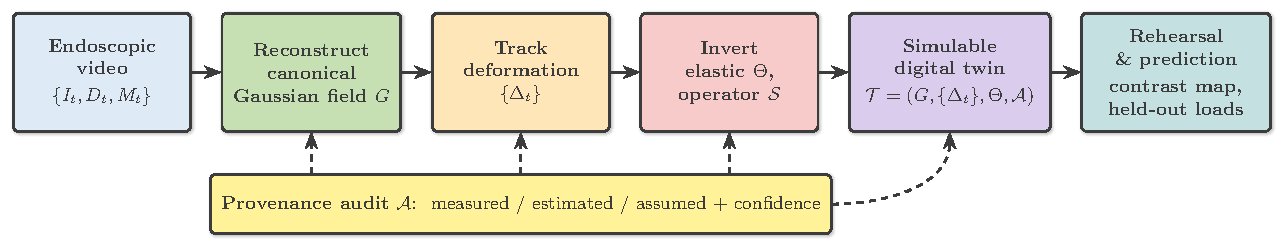
\includegraphics[width=\textwidth]{fig_pipeline.pdf}
\caption{Overall pipeline for converting a monocular endoscopic
video into a soft-tissue digital twin that can be driven forward in a
physics simulator. Reconstruction fits a canonical Gaussian field $G$
from the reference frame; tracking estimates the deformation sequence
$\{\Delta_t\}$ on that fixed set of primitives; and mechanical inversion
recovers the elastic parameters
$\Theta$ and the forward operator $\mathcal{S}$ by differentiable
simulation. The provenance audit $\mathcal{A}$ accompanies the result, tagging
every physical parameter as measured, estimated, or assumed and attaching
an uncertainty estimate.}
\label{fig:pipeline}
\end{figure*}

Potential applications include simulation-based rehearsal of tissue
manipulation, haptic training, and prediction of deformation outside the
endoscopic field of view. These applications require not only geometric
and appearance fidelity but also mechanically supportable parameter
estimates with quantified uncertainty.

The core difficulty is that geometry and appearance are observable from
images, while mechanical parameters (Young's modulus $E$, Poisson ratio
$\nu$, viscosity) are not. Radiance measurements do not directly identify
stress or elasticity. A
mechanical parameter can only be obtained in two ways: (a) it is looked up
from a tissue-class prior (an assumption), or (b) it is inferred by
observing deformation under known loading (a measurement, subject to the
identifiability limits of the loading). Prior reconstruction studies
generally prescribe mechanical constants without quantifying their
evidential basis. Predictions obtained with such constants cannot be
interpreted as patient-specific mechanical estimates. Accordingly, the
proposed twin records whether each parameter was measured, estimated, or
assumed \cite{topol2019,landig2025}.

\subsection{Related work}
\label{sec:related}
%% ===================================================================

Table~\ref{tab:position} summarizes representative methods in medical
digital twins, endoscopic reconstruction, and physics-based system
identification.

\begin{table*}[htbp]
\centering
\caption{Functional comparison with representative related methods.}
\label{tab:position}
\footnotesize
\begin{tabular}{@{}p{0.16\linewidth}p{0.20\linewidth}p{0.16\linewidth}p{0.16\linewidth}p{0.16\linewidth}@{}}
\toprule
Method & Output & Mechanics & Provenance & Validated on \\
\midrule
EndoNeRF \cite{endonerf} & appearance, geometry & none & none & EndoNeRF \\
EndoSurf \cite{endosurf} & surface, appearance & none & none & stereo endoscopy \\
EndoGaussian \cite{endogaussian} & appearance, geometry & none & none & EndoNeRF \\
PAC-NeRF \cite{pacnerf} & geometry, system identification & $E$, known force & implicit & synthetic data, objects \\
PhysDreamer \cite{physdreamer} & relative stiffness & relative $E$ & implicit & static objects \\
PhysGaussian \cite{physgaussian} & dynamics & material point method (MPM), manual $E$ & none & synthetic \\
\textbf{Present method} & \textbf{simulable twin} & $E$, $\nu$, viscosity & \textbf{explicit audit} & \textbf{EndoNeRF; SCARED; FEM; phantom} \\
\bottomrule
\end{tabular}
\end{table*}

\subsubsection{Medical digital twins}
Digital twins originated in industry, where a constantly updating virtual
copy enables analysis, simulation, and prediction of a real-world asset
\cite{tao2019,fuller2020}, and are increasingly studied as a route to
precision medicine. Recent frameworks decompose a medical twin into the
patient, the data connection, the patient-in-silico model, the interface,
and twin synchronisation \cite{landig2025,laubenbacher2024}. The
cardiology community has produced the most mature examples, with
electrophysiology heart twins used to plan ablation and resynchronization
therapy; oncology has produced tumor-growth twins coupling imaging with
reaction--diffusion models; and epidemiology has produced population-level
twins for policy testing. These share a common structure (a mechanistic
or learned patient-in-silico model synchronized with patient data) but
their state variables are compartmental, hemodynamic, or cellular rather
than mechanical. Intra-operative soft-tissue twins built from endoscopic
video remain largely unexplored. Existing frameworks also do not specify
the provenance of individual physical parameters. The present method
incorporates a measured/estimated/assumed audit and uses the tracking loop
(Sec.~\ref{sec:sync}) for twin synchronisation \cite{landig2025}.

\subsubsection{Endoscopic scene reconstruction}
EndoNeRF \cite{endonerf} introduced neural radiance fields \cite{nerf}
for deformable endoscopic scenes, demonstrating novel-view synthesis of
tissue deformation by conditioning a radiance field on a learned
deformation code per frame. EndoSurf \cite{endosurf} improved surface
fidelity by combining a neural signed-distance field with a surface-aware
rendering loss, yielding cleaner tissue boundaries. A line of
Gaussian-splatting methods \cite{gaussiansplatting}, including EndoGaussian
\cite{endogaussian}, replaced
the implicit field with anisotropic 3D Gaussians, gaining an order of
magnitude in rendering speed and enabling per-primitive appearance. These
methods reconstruct appearance and geometry but do not recover physical
parameters, and their output cannot be loaded into a physics simulator.
Complementary lines address camera tracking and mapping in endoscopy, from
stereo correspondence \cite{scared} and robust pose estimation
\cite{hayoz2023} to deformable SLAM \cite{defslam}, and inverse-rendering
methods recover relightable appearance with bidirectional reflectance
distribution function (BRDF) decomposition
\cite{gsir2024,relightable3dgs}, but do not estimate mechanical parameters.
The present reconstruction uses the Gaussian representation with a
constrained BRDF (Sec.~\ref{sec:tier1}); the same field is subsequently
tracked and mechanically parameterized. Tool-aware masking restricts
supervision to tissue pixels and improves the corresponding ablation by
${\sim}25$\,dB.

\subsubsection{Physics-aware reconstruction}
A growing line of work couples neural reconstruction with physics.
PAC-NeRF \cite{pacnerf} performs system identification from multi-view
video with known forces, recovering material parameters of household
objects by matching a differentiable continuum simulator to observed
motion; its key requirement is a measured force, which is rarely available
in endoscopy. PhysDreamer \cite{physdreamer} uses a video diffusion prior
to estimate the relative stiffness of static objects, trading absolute
accuracy for the ability to work from a single video. PhysGaussian
\cite{physgaussian} embeds the Material Point Method into Gaussians for
generative dynamics but requires manually supplied material parameters, so
the physics is imposed rather than recovered. Spring-Gaus and similar
variants attach spring models to Gaussians for elastic dynamics
\cite{springgaus,physicallyembodied}, and graph-network simulators learn
complex physics from data \cite{sanchezgonzalez2020}. These works
demonstrate that physics can be coupled with learned reconstruction, but
they either assume known forces, recover only relative stiffness, or
require manual parameters. None of the compared methods reports
per-parameter provenance. The present method targets endoscopic soft tissue,
recovers absolute modulus when the applied load is known, and records the
provenance of every parameter. Proposition~\ref{prop:forcescale} shows why
the force scale constrains absolute-modulus recovery.

\subsubsection{Elastography}
Quasi-static elastography recovers modulus contrast from deformation under
a shared-stress approximation \cite{ophir1991,wells2011,sigrist2017}, and
is clinically established for liver fibrosis staging and tumor detection.
The method tracks the axial strain induced by a small compression; under
the assumption that the stress is approximately uniform across a region,
the ratio of strains in two regions approximates the inverse ratio of their
moduli, so a stiff inclusion appears as a low-strain region. Without a
force measurement, this approximation identifies contrast rather than
absolute modulus. Proposition~\ref{prop:forcescale} provides the
corresponding force-scale relation, and the audit therefore reports
contrast when the force magnitude is unavailable.

\subsubsection{Differentiable simulation and uncertainty}
Differentiable physics (differentiable FEM, MPM, and mass--spring
solvers) enables gradient-based parameter inversion through a simulator
\cite{pacnerf,physgaussian,hu2020difftaichi,sanchezgonzalez2020}. We use a
differentiable Neo-Hookean FEM for the main inversion and a fast
mass--spring surrogate for synthetic closed-loop studies, and we quantify
the surrogate's inadequacy (82\% forward error) to justify the FEM choice.
Laplace approximations and Monte-Carlo propagation are established
uncertainty methods \cite{kendall2017,gal2016,lakshminarayanan2017}. Here
they are used to identify weakly constrained parameters and to propagate
parameter uncertainty to predicted displacement.

\subsubsection{Methodological gap}
\label{sec:gaps}
The remaining gap is a co-registered framework that connects endoscopic
reconstruction and temporally consistent surface displacement to
mechanical parameterization while distinguishing measured quantities from
prior assumptions. The proposed Gaussian field supplies the surface
observations, differentiable Neo-Hookean inversion supplies the
known-force mechanics, and the provenance map records their evidential
status. Evaluation ranges from a synthetic closed loop to a physical
phantom with independent compression measurements.

Based on 3D Gaussian splatting \cite{gaussiansplatting} and differentiable
Neo-Hookean finite elements \cite{holzapfel2000,hu2020difftaichi}, we
propose an audited soft-tissue digital twin
$\mathcal{T}=(G,\{\Delta_t\},\Theta,\mathcal{A})$
(Fig.~\ref{fig:pipeline}, Fig.~\ref{fig:architecture}).

The representation couples appearance and motion through a canonical field
of anisotropic Gaussians. Each primitive stores geometry and a constrained
Cook--Torrance reflectance model \cite{cooktorrance}. Instrument-excluded,
depth-valid supervision fits this field, and fixed primitive identities
provide correspondences for estimating displacement over time.
Constant-velocity initialization, graph regularization, and rollback after
divergence stabilize the tracked displacement.

Mechanical parameterization is conditioned on the available force
evidence. For uninstrumented endoscopic sequences, tracked Gaussians are
partitioned into spatial regions and their mean displacement magnitudes
provide a common-load relative-stiffness estimate; no absolute modulus is
assigned from video. For benchmark cases with known forces, surface
displacements are compared with a differentiable tetrahedral FEM solution,
and Young's modulus is recovered by implicit differentiation of
quasi-static equilibrium. The Gaussian field and tetrahedral mesh are
separate discretizations coupled through surface-displacement
observations. Thus, the shared representation refers to co-registration of
appearance, motion, and regional mechanical metadata rather than use of
Gaussian primitives as FEM elements.

The force-scale analysis formalizes the corresponding identifiability
limit. At fixed Poisson ratio, scaling all regional moduli and the applied
force by the same factor leaves equilibrium displacement unchanged
(Proposition~\ref{prop:forcescale}); absolute modulus therefore inherits
force-scale uncertainty, whereas regional stiffness contrast does not.
An R3D-18 retraction-force estimator from unpublished experiments supplies
an empirical force-error model for sensitivity analysis.

A log-normal Bayesian update records each parameter as measured, estimated,
or assumed and propagates posterior uncertainty through the simulator
(Sec.~\ref{sec:uq}). Direct sensor observations are measured,
reconstruction or inverse-simulation outputs are estimated, and
table-derived values without case-specific evidence are assumed.

The methodological novelty lies in the observation-to-simulation
interface: fixed-identity Gaussians provide co-registered appearance and
surface motion; force-scale analysis determines whether absolute modulus
or only relative contrast is identifiable; and the provenance map preserves
that distinction in the resulting twin. The individual renderer,
constitutive model, and Bayesian update are established techniques; their
coupling and identifiability-aware reporting are the contribution of this
study.

The study additionally derives one patient-specific liver mesh from 82
de-identified abdominal computed tomography (CT) slices. Mechanical ground
truth is provided by a finite-element method (FEM) benchmark of 60
scenarios and four load cases, of which six
are inverted in this study. Evaluation proceeds from a synthetic
closed loop to a physical ultrasound phantom with compression-test
measurements (Sec.~\ref{sec:experiments}).

Across two EndoNeRF scenes and the SCARED stereo dataset, reconstruction
recovers tissue at 26.6--36.8\,dB tissue-masked peak signal-to-noise ratio
(PSNR). Tracking follows the deformation where inertia-only tracking
diverges. Mechanical inversion recovers uniform modulus to 0.01\% error in a
synthetic closed loop, background modulus to a median of 4.3\% error on an
independent FEM benchmark, and modulus contrast to 6.9\% error on a real
ultrasound phantom with independent compression-test ground truth.
Absolute modulus is not reported for real tissue in the absence of force
sensing, and the reconstruction results are not treated as a novel-view
synthesis comparison.

The rest of the paper follows the journal's structure:
Section~\ref{sec:experiments} reports the results,
Section~\ref{sec:discussion} discusses implications and limitations,
Section~\ref{sec:method} details the methods, and
Section~\ref{sec:conclusion} concludes.

%% ===================================================================

\section{Results}
\label{sec:experiments}
%% ===================================================================

Reconstruction and tracking are reported on endoscopic and stereo video.
Mechanical inversion is then reported as the force evidence changes, from
a known load, to a video-based force estimate, to no force measurement.
Uncertainty, comparison with related methods, and ablations follow.
Limitations are discussed with the clinical implications.

\begin{figure*}[htbp]
\centering
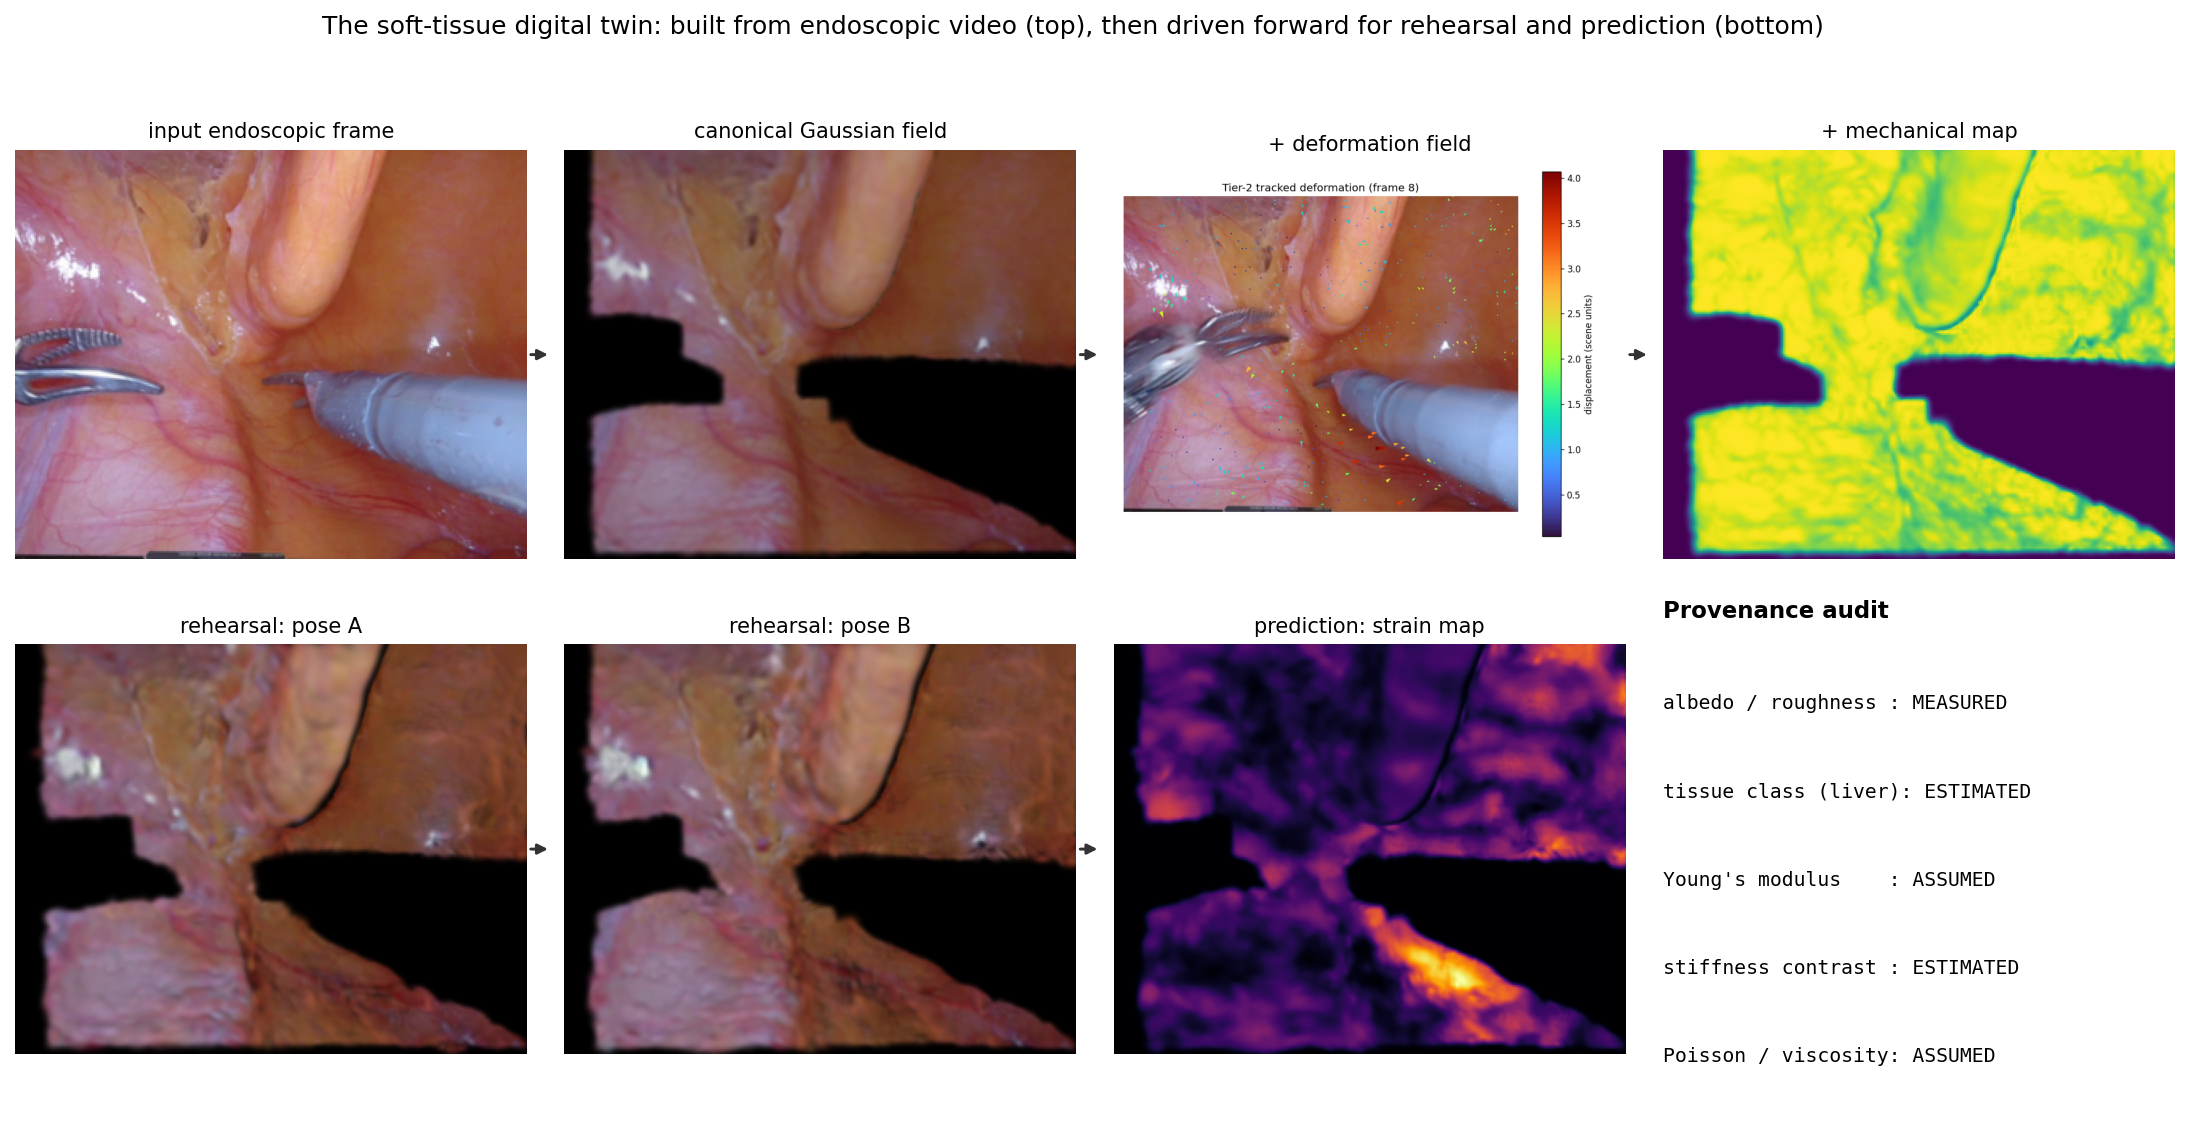
\includegraphics[width=\textwidth]{fig_twin_complete.png}
\caption{The soft-tissue digital twin, end to end. \emph{Top (building the
twin):} from an input endoscopic frame, the pipeline reconstructs the
canonical Gaussian field, tracks the deformation field on it, and attaches a
mechanical parameter map. \emph{Bottom (using the twin):} the twin is then
driven forward in the simulator to rehearsal poses, produces a strain
prediction, and reports a provenance audit that tags every parameter as
measured, estimated, or assumed. The figure summarizes the
input$\to$twin$\to$output relation evaluated below.}
\label{fig:twin_complete}
\end{figure*}

\subsection{Canonical reconstruction}
The fitted Gaussian field is the representation that tracking and inversion
reuse, so its tissue fidelity is reported first.
\begin{table*}[htbp]
\centering
\caption{Reconstruction (tissue-masked PSNR).}
\label{tab:tier1}
\footnotesize
\begin{tabular}{lcccc}
\toprule
Scene & Frames used & Tissue coverage & Gaussians & Tissue PSNR (dB) \\
\midrule
EndoNeRF pulling & 16--24 & 70.7\% & 6498 & \textbf{36.79} \\
EndoNeRF cutting & 16--24 & 74.1\% & 6824 & \textbf{34.09} \\
SCARED keyframe\_1 & 1 & 78.4\% & 7221 & 26.99 \\
SCARED keyframe\_2 & 1 & 83.1\% & 7676 & 26.17 \\
\bottomrule
\end{tabular}
\end{table*}

\begin{table*}[htbp]
\centering
\caption{Reconstruction protocols. Novel-view numbers from
EndoNeRF \cite{endonerf}, EndoSurf \cite{endosurf}, and
EndoGaussian \cite{endogaussian} are not copied here, because this paper
did not re-run that split and the public reports do not all quote the same
aggregate. The two rows below are tissue-masked fits of the canonical
field, not held-out novel views.}
\label{tab:recon_compare}
\small
\begin{tabular}{@{}p{0.36\textwidth}p{0.42\textwidth}p{0.12\textwidth}@{}}
\toprule
Method & Protocol & PSNR (dB) \\
\midrule
EndoNeRF, EndoSurf, EndoGaussian & novel-view synthesis (NVS), held-out views & not re-run \\
\midrule
\textbf{Present study (pulling)} & canonical, tissue-masked & \textbf{36.79} \\
\textbf{Present study (cutting)} & canonical, tissue-masked & \textbf{34.09} \\
\bottomrule
\end{tabular}
\end{table*}

All-image PSNR is lower by design because tools are masked out and not
reconstructed; we report tissue-masked PSNR throughout.
Table~\ref{tab:tier1} reports per-scene reconstruction quality, and
Fig.~\ref{fig:tier1} shows the corresponding reconstructions. The higher
PSNR in the pulling scene coincides with greater tissue coverage and more
uniform illumination. In both EndoNeRF scenes, the largest errors occur
near the instrument--tissue boundary. Each SCARED keyframe is fitted from
one view without multi-frame supervision; these experiments assess
transfer to a different anatomy, camera, and metric scale
(Fig.~\ref{fig:tier1}).

\begin{figure}[htbp]
\centering
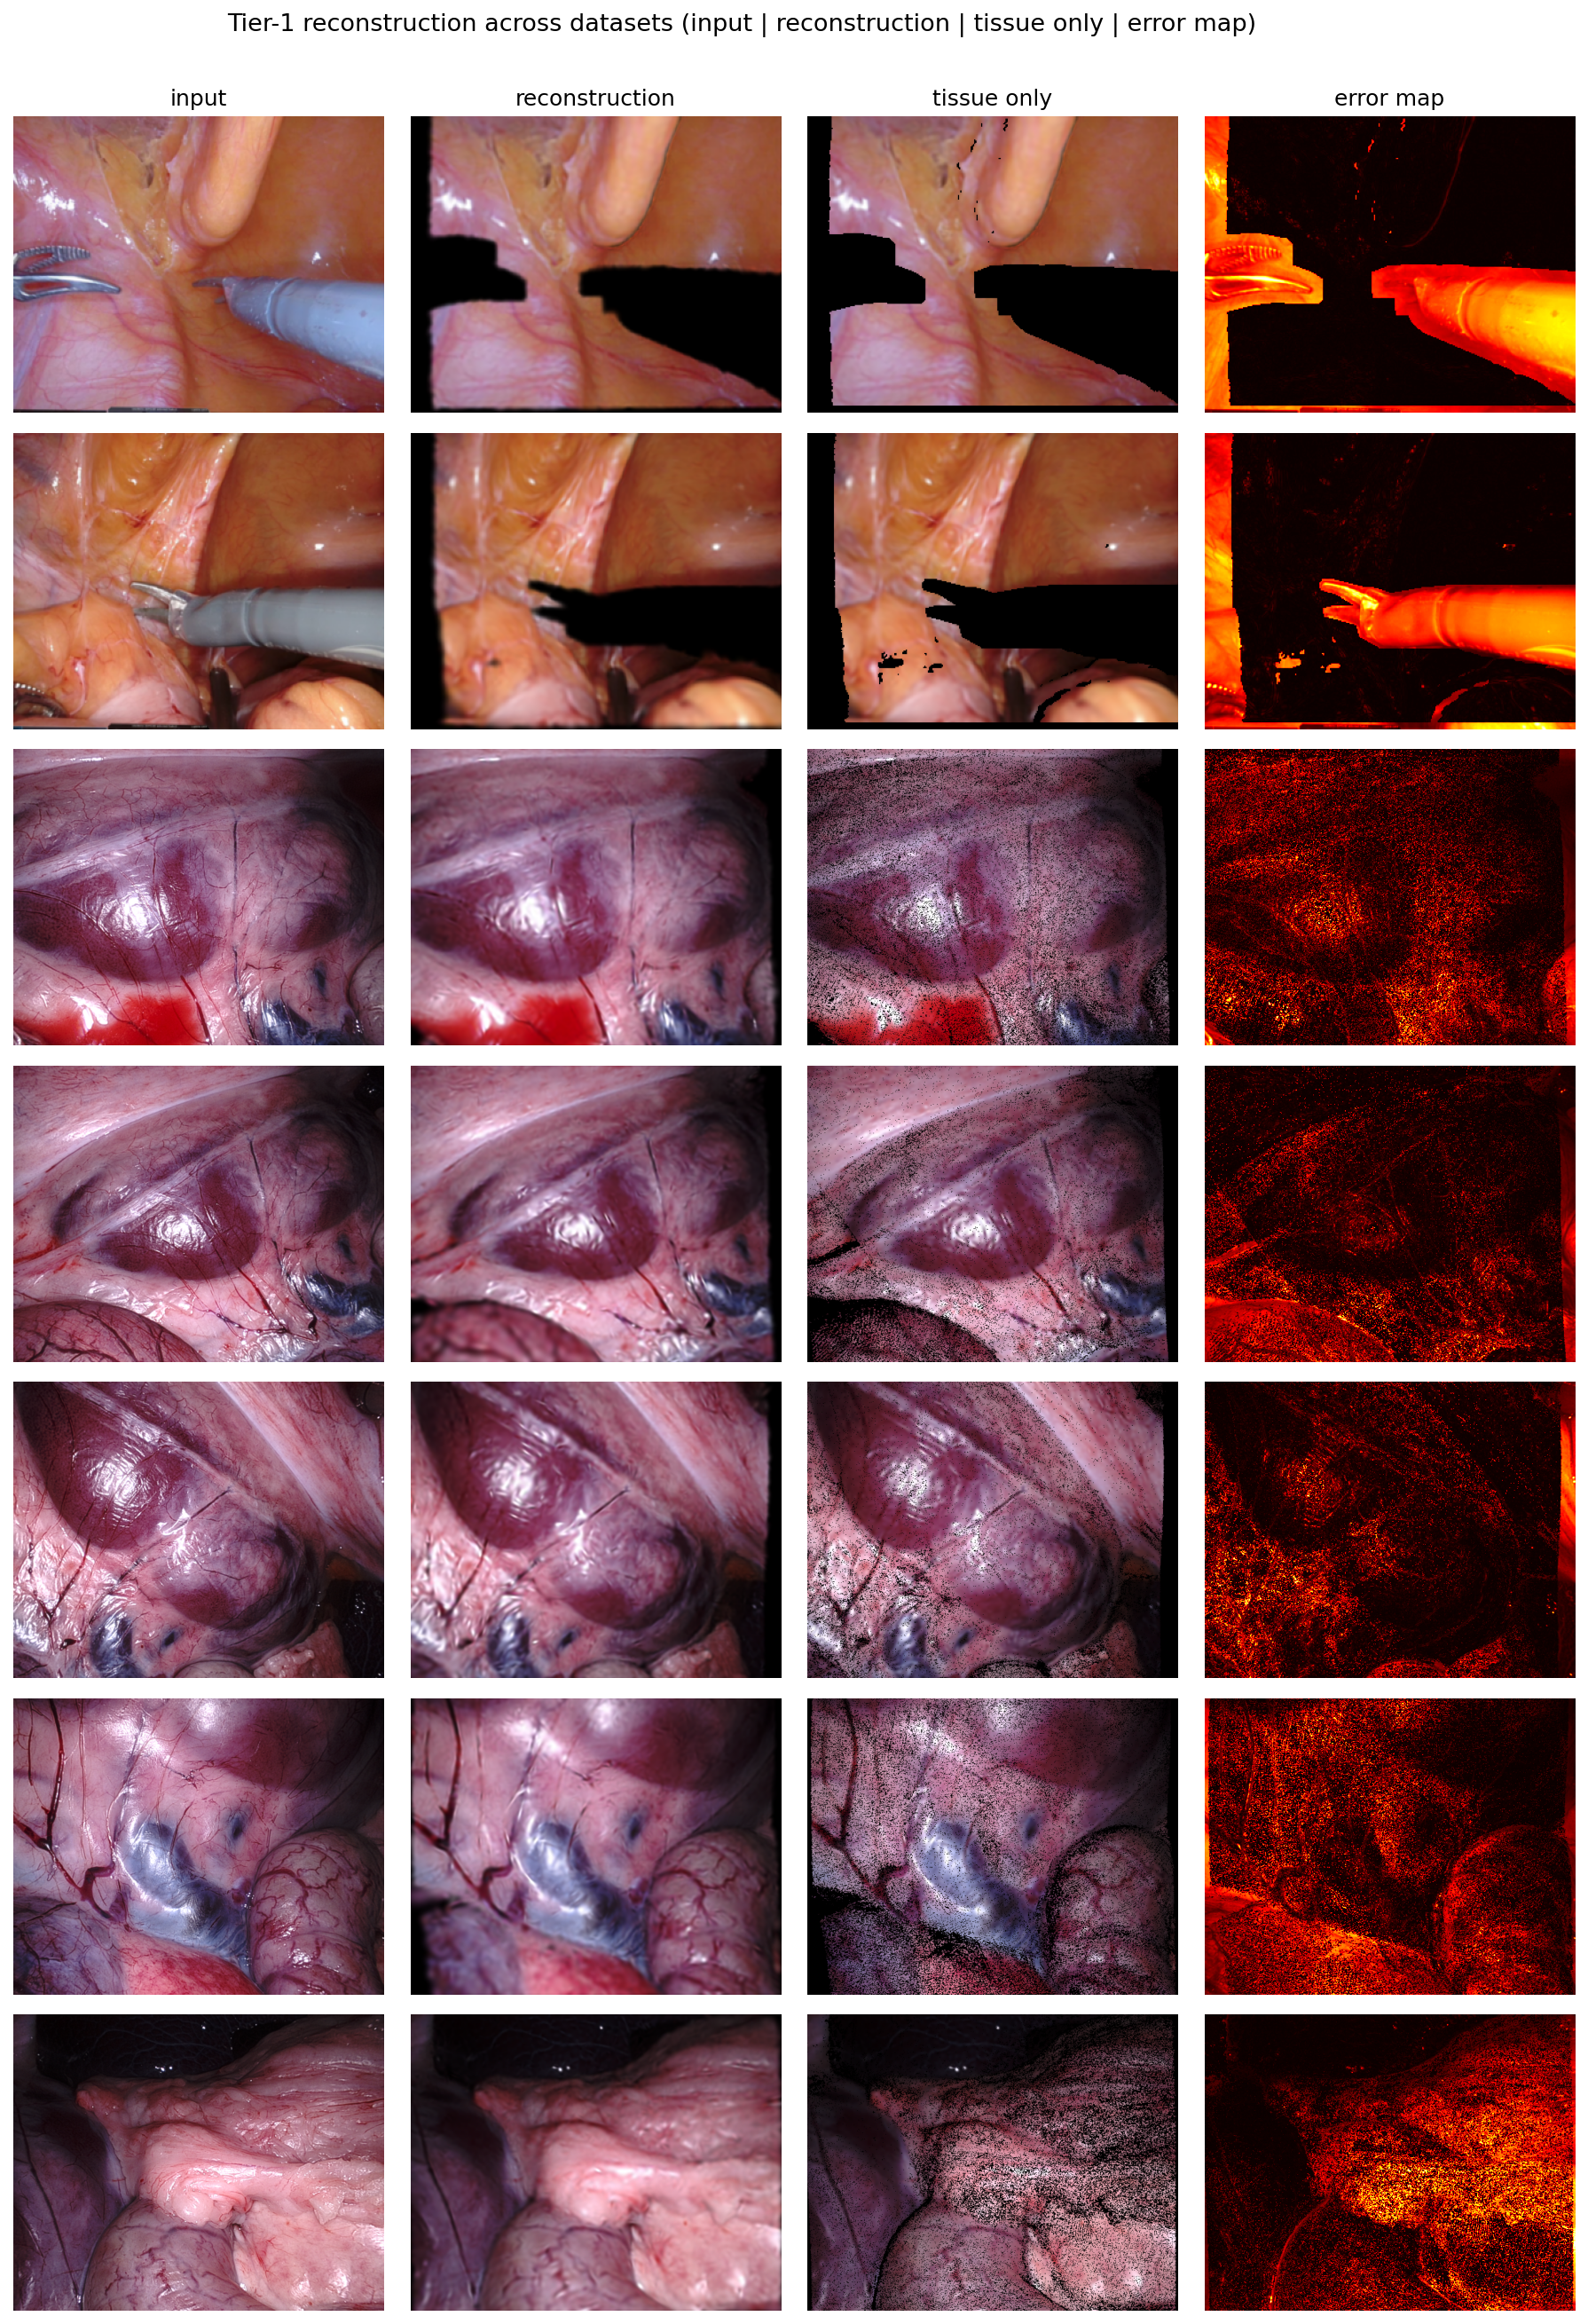
\includegraphics[width=\linewidth]{fig_recon_grid.png}
\caption{Qualitative reconstruction. Rows are EndoNeRF pulling, EndoNeRF
cutting, and SCARED keyframes. Columns are input, reconstruction, tissue
only, and an error map. Tissue-masked PSNR is reported in
Table~\ref{tab:tier1} for the two EndoNeRF scenes and SCARED keyframes 1
and 2. The remaining SCARED rows are shown only as a visual check; they
are not given a separate PSNR in this paper.}
\label{fig:tier1}
\end{figure}

\subsection{Deformation tracking}
Tracking attaches a displacement to each primitive of the field fitted
above. Fixed primitive identities are what allow the sequence to be used
as a boundary condition.
\begin{table}[htbp]
\centering
\caption{Temporal-model ablation (pulling scene).}
\label{tab:tier2}
\small
\begin{tabular}{lcc}
\toprule
Tracker & Worst-frame loss & Behaviour \\
\midrule
Inertia-only & 37.23 & frame 5 divergence \\
Const-vel + rollback & 1.55 & frame 5 rolled back \\
\bottomrule
\end{tabular}
\end{table}

Fig.~\ref{fig:tier2} shows the tracked deformation field; displacement
concentrates at the tool contact region. Table~\ref{tab:tier2} ablates the
temporal model: the inertia-only baseline fails on
frame 5 of the pulling scene. This failure coincides with a fast, partially
occluded retraction and a weak local photometric gradient. Constant-velocity
initialization and acceleration regularization avoid divergence, while
rollback prevents the failed update from propagating to the next frame.
On the cutting scene the same tracker runs
six frames without divergence (loss 0.52--0.71). The tracked displacements
are the observations passed to the mechanical inversion.

\begin{figure}[htbp]
\centering
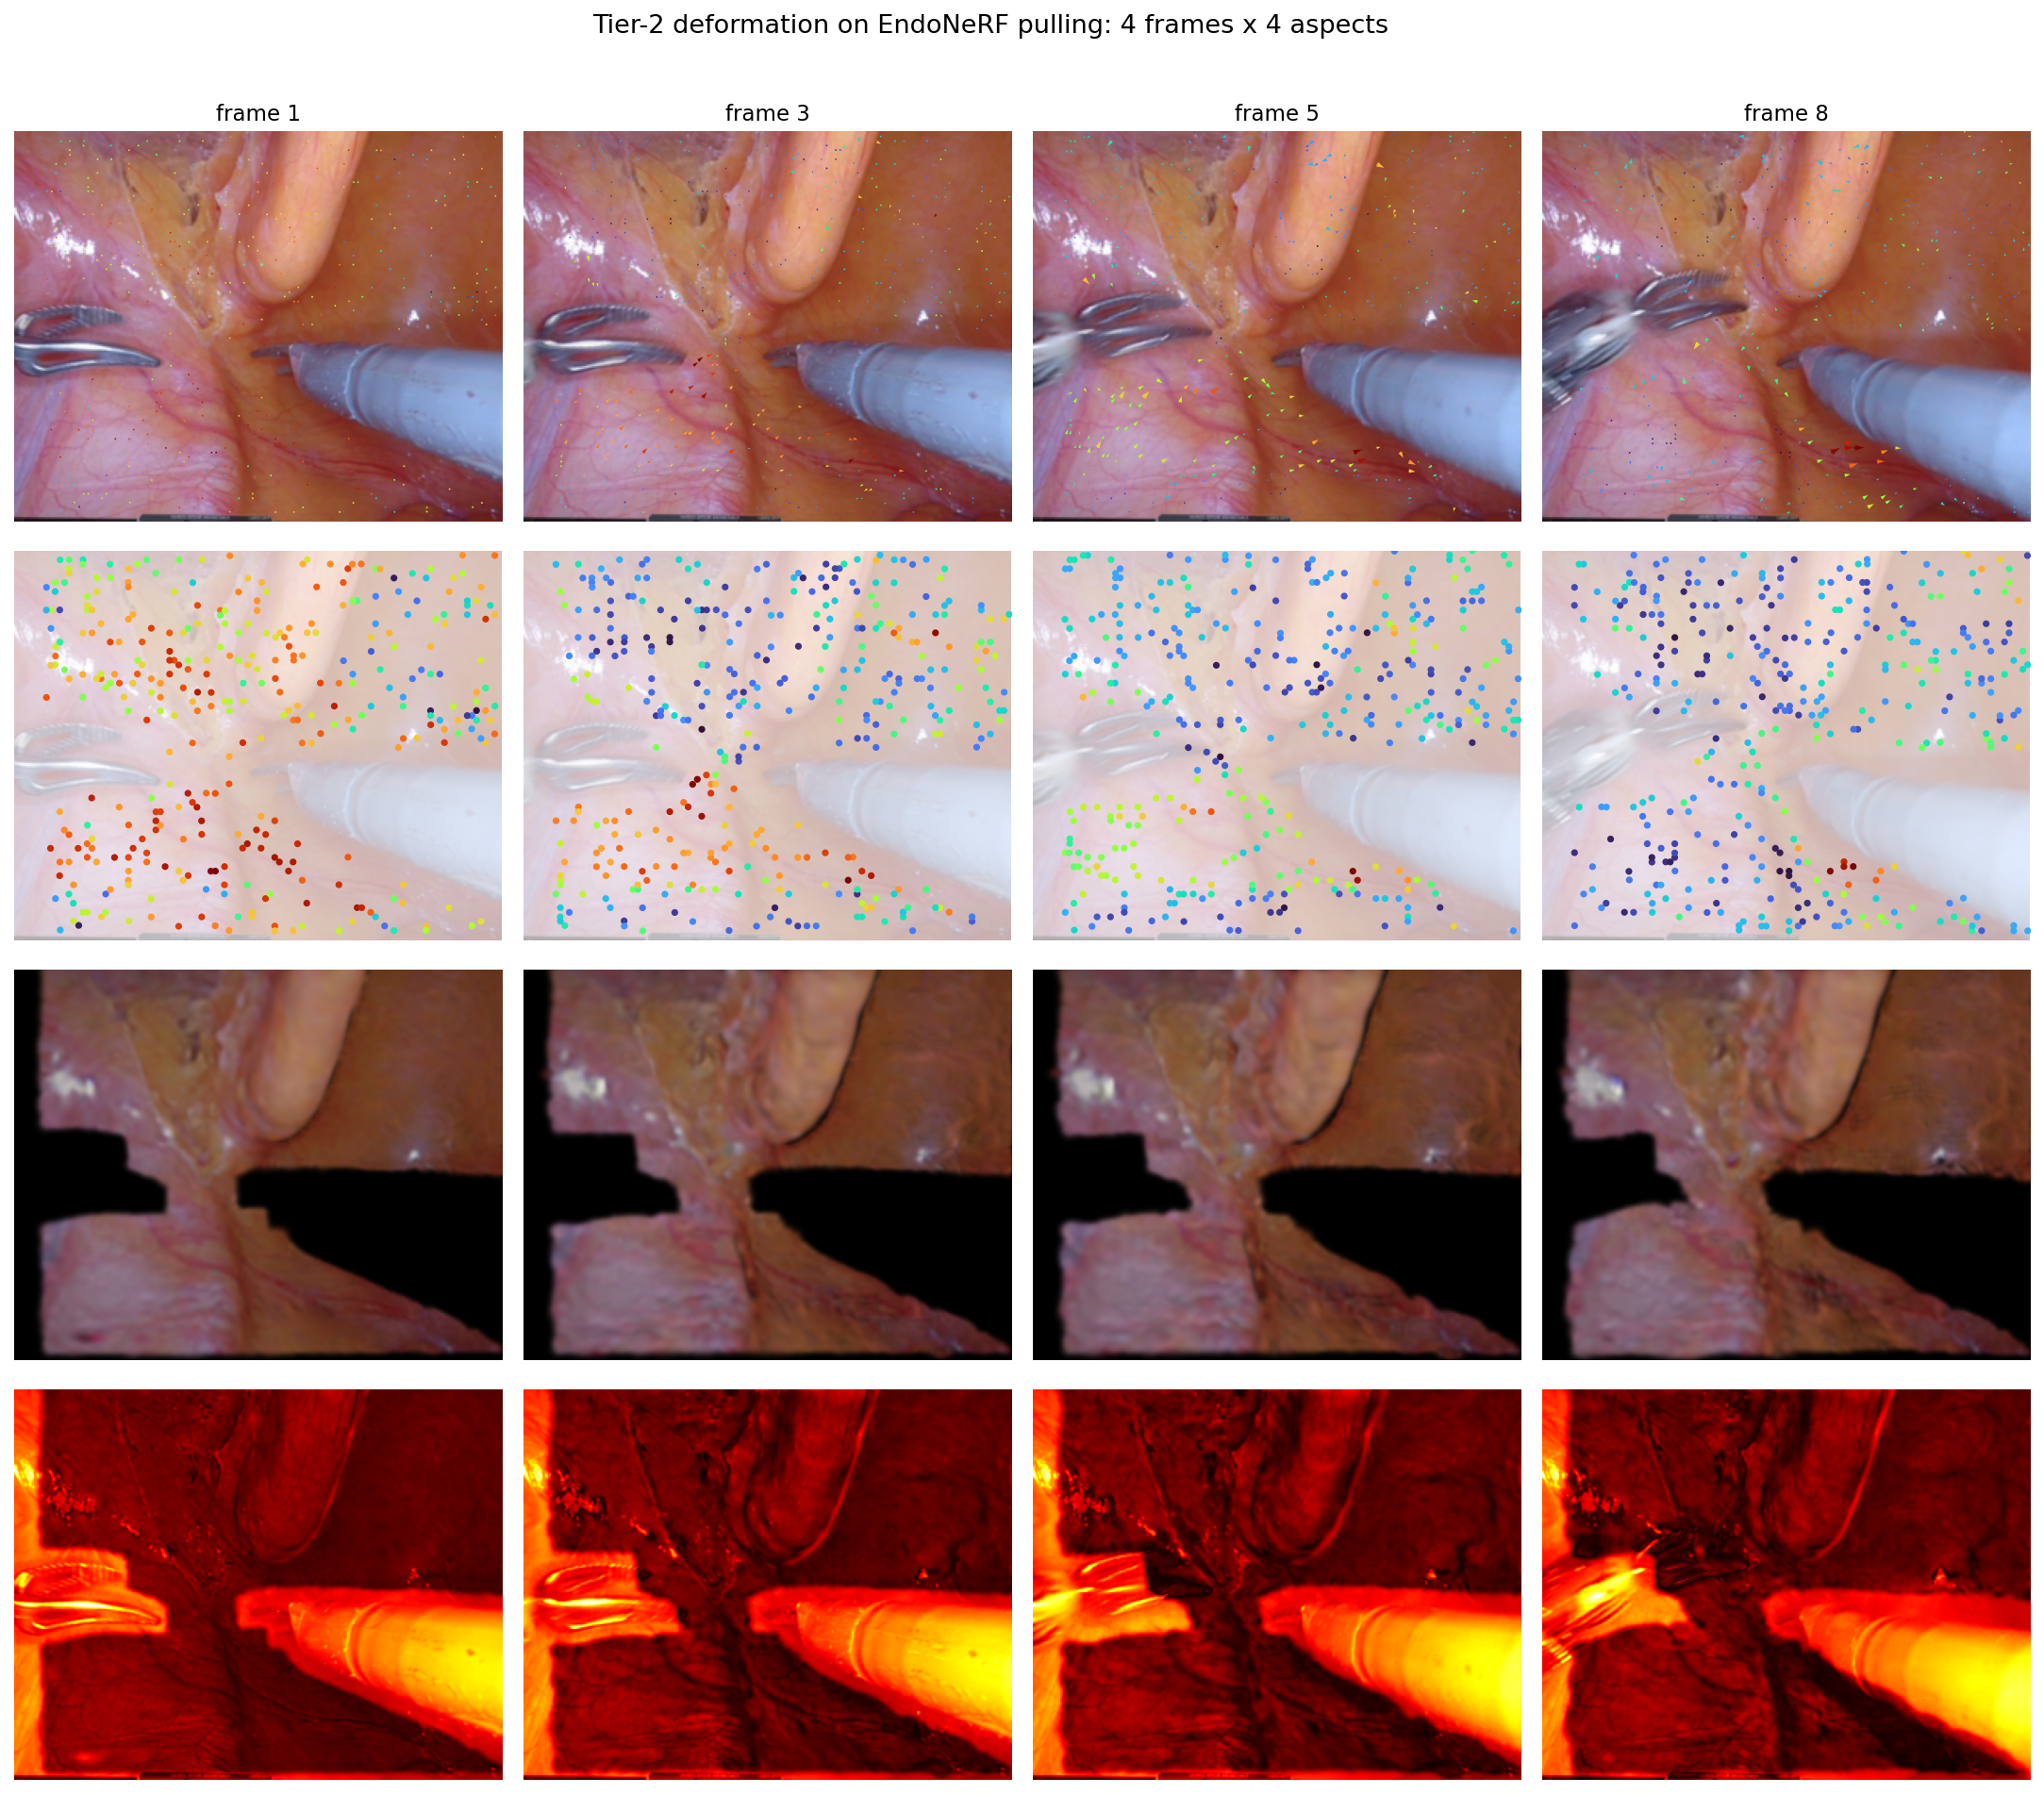
\includegraphics[width=\linewidth]{fig_deform_4x4.png}
\caption{Deformation on EndoNeRF pulling, four frames (columns)
$\times$ four aspects (rows): quiver overlay, displacement-magnitude
heatmap, deformed-field render, and photometric error map. The tracked
displacement grows and localizes at the tool contact, and the deformed
render matches the observed frame.}
\label{fig:tier2}
\end{figure}

\subsection{Mechanical inversion}
Table~\ref{tab:ladder} summarizes inversion as the force evidence changes:
a known load, a video-based force estimate, and no force measurement.
For the EndoNeRF sequences, tracked Gaussians produce a four-region
relative-stiffness field through Eq.~\eqref{eq:relative_stiffness}. Because
these sequences provide neither force measurements nor stiffness
references, this output is not assigned an absolute scale and is not used
as a quantitative validation result. Absolute-modulus validation is
performed on the force-calibrated FEM benchmark, and contrast validation is
performed on the compression-tested phantom.

\begin{table*}[htbp]
\centering
\caption{Mechanical inversion under successively weaker force evidence.
The remaining rows are additional checks on the finite-element benchmark.}
\label{tab:ladder}
\small
\begin{tabular}{@{}p{0.27\linewidth}p{0.32\linewidth}p{0.29\linewidth}@{}}
\toprule
Setting & Evidence & Result \\
\midrule
Synthetic closed loop (mass--spring) & uniform $E$ & 0.01\% error \\
Synthetic inclusion (mass--spring) & $4.0\times$ contrast, surface-only & $3.19\times$ \\
Independent FEM benchmark & $E_{bg}$, measured force; noisy motion & \textbf{median 4.3\% error (6 scenarios)} \\
Held-out load case (FEM) & press\_left $\rightarrow$ other cases & within 4.1\% of oracle \\
Noise robustness (FEM) & +0.5 / +1.0\,mm noise & $E_{bg}$ error 13--20\% / 9--23\% \\
Surrogate comparison & mass--spring versus FEM & 82\% error $\Rightarrow$ FEM retained \\
Posterior width & Laplace approximation & inclusion flagged unidentified \\
Force provenance & unpublished video-force error $\rightarrow$ $E$ & $E_{bg}$ 4.1$\pm$4.0\%; contrast unchanged \\
\textbf{Real phantom (\'ETS)} & contrast versus compression-test reference & \textbf{6.9\% error; 95\% confidence interval includes reference} \\
\bottomrule
\end{tabular}
\end{table*}

\paragraph{Synthetic closed loop}
Uniform modulus is recovered to 0.01\% error; a $4\times$ stiff inclusion
is recovered at $3.19\times$ contrast from surface-only observations with
two load cases (Fig.~\ref{fig:tier3}).

\begin{figure}[htbp]
\centering
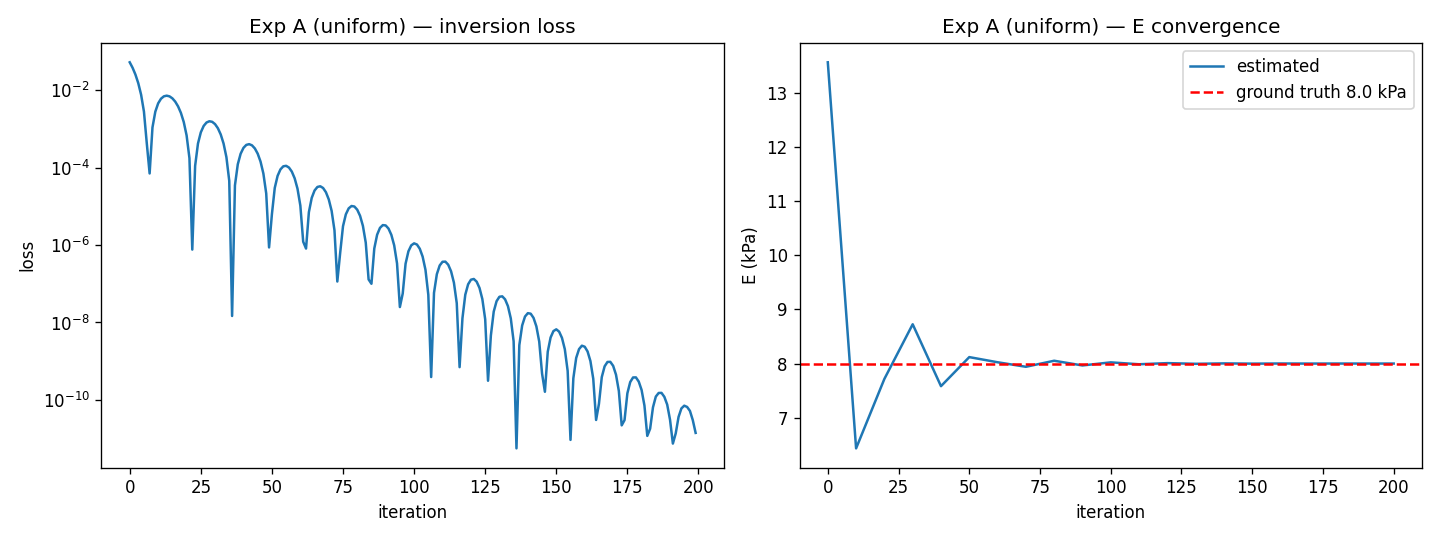
\includegraphics[width=0.49\linewidth]{fig_tier3_uniform.png}
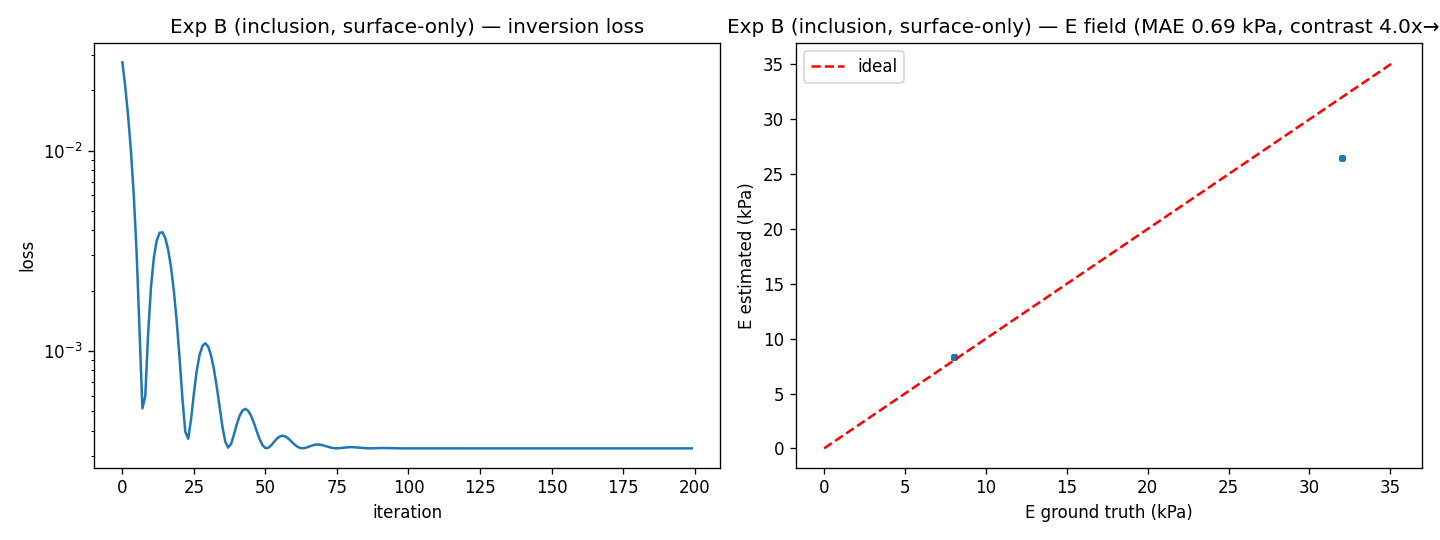
\includegraphics[width=0.49\linewidth]{fig_tier3_inclusion.png}
\caption{Synthetic closed loop: (left) uniform $E$ converges to the
8.0\,kPa ground truth; (right) stiff-inclusion contrast $4.0\times$ $\to$
$3.19\times$.}
\label{fig:tier3}
\end{figure}

\paragraph{Independent FEM benchmark}
With measured forces (5\% calibrated error) and noisy surface motion, the
background modulus is recovered to a median error of 4.3\% (mean 9.4\%)
across six scenarios drawn from the 60-scenario benchmark
(per-scenario values in
Table~\ref{tab:perscenario}). Error is below 6\% for the four cases with
$E_{bg} \ge 3.8$\,kPa and reaches 17--27\% for the two cases with the
lowest background moduli. The six-case analysis is insufficient to
identify the cause of this association. The inclusion contrast is
recovered to a mean of $1.90\times$
against a ground-truth mean of $2.41\times$. Material inverted on
\texttt{press\_left} predicts unseen load cases with displacement error
11.1\% (\texttt{press\_right}), 3.7\% (\texttt{shear\_x}), and 14.9\%
(\texttt{shear\_y}), against oracle-material errors of 9.6\%, 7.2\%, and
10.9\% respectively (Fig.~\ref{fig:fem_perscenario},
Fig.~\ref{fig:fem_dist}, and the robustness summary in
Fig.~\ref{fig:robustness}).

\begin{table}[htbp]
\centering
\caption{Per-scenario FEM-benchmark background-modulus inversion.}
\label{tab:perscenario}
\small
\begin{tabular}{lcccc}
\toprule
Scenario & $E_{bg}^{gt}$ (kPa) & $E_{bg}^{est}$ (kPa) & Error (\%) & Estimated/true contrast \\
\midrule
000 & 7.35 & 7.24 & 1.6 & $2.26\times / 1.71\times$ \\
001 & 2.61 & 2.17 & 17.1 & $2.09\times / 2.79\times$ \\
002 & 3.81 & 3.90 & 2.3 & $1.34\times / 3.66\times$ \\
003 & 7.78 & 7.54 & 3.1 & $1.30\times / 1.00\times$ \\
004 & 2.81 & 2.05 & 26.9 & $2.00\times / 1.30\times$ \\
005 & 4.57 & 4.82 & 5.5 & $2.38\times / 3.99\times$ \\
\midrule
\multicolumn{3}{l}{median / mean error} & 4.3 / 9.4 & mean $1.90\times / 2.41\times$ \\
\bottomrule
\end{tabular}
\end{table}

\begin{figure}[htbp]
\centering
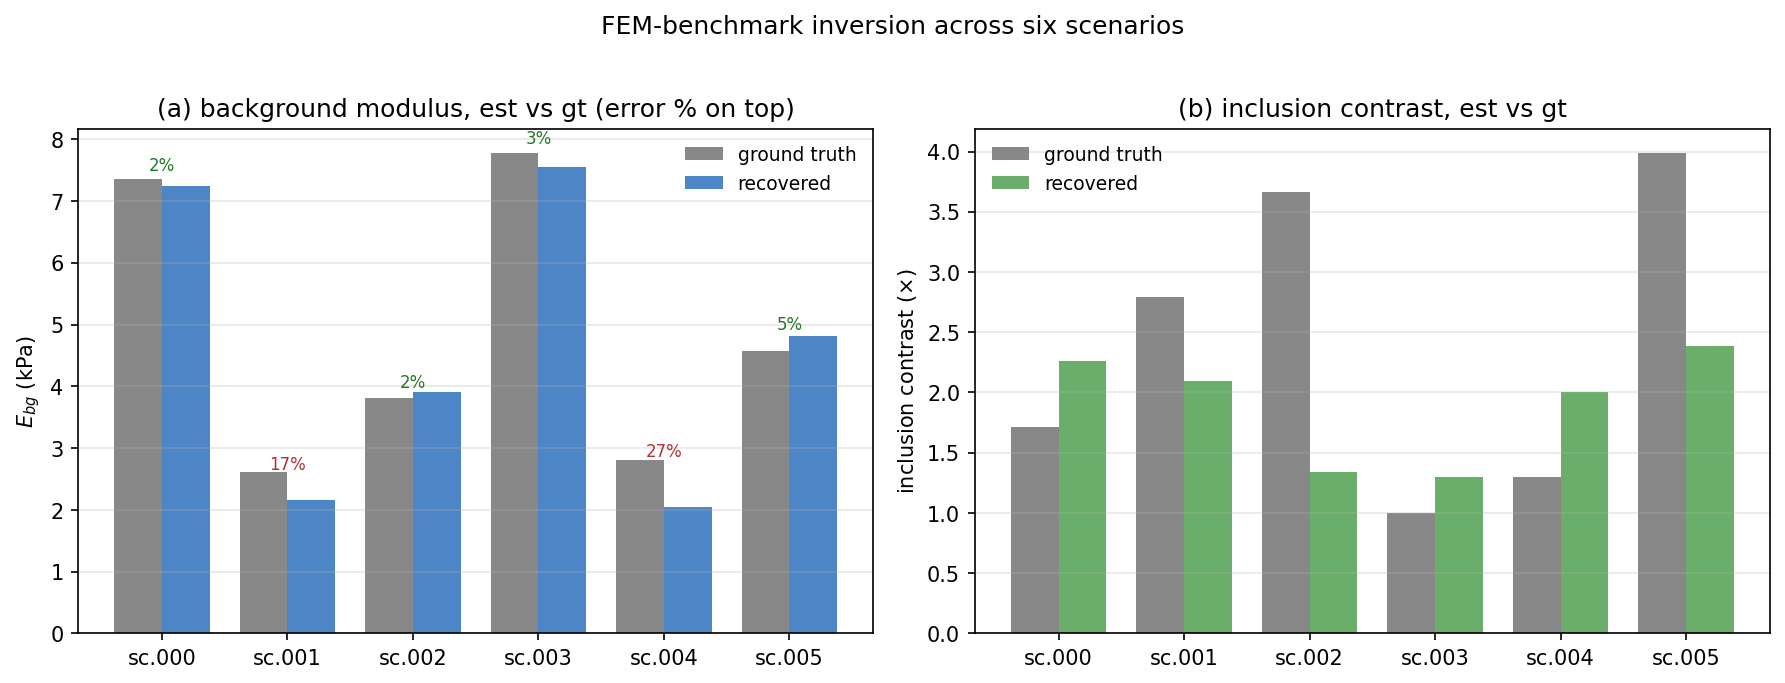
\includegraphics[width=\linewidth]{fig_fem_perscenario.png}
\caption{Per-scenario FEM-benchmark inversion. (a) Background modulus,
recovered vs ground truth, with the relative error annotated (green $<10\%$,
red $>10\%$). (b) Inclusion contrast, recovered vs ground truth. The two
softest backgrounds (sc.\ 001, 004) are the hardest, consistent with the
regime-dependence analysis.}
\label{fig:fem_perscenario}
\end{figure}

\begin{figure}[htbp]
\centering
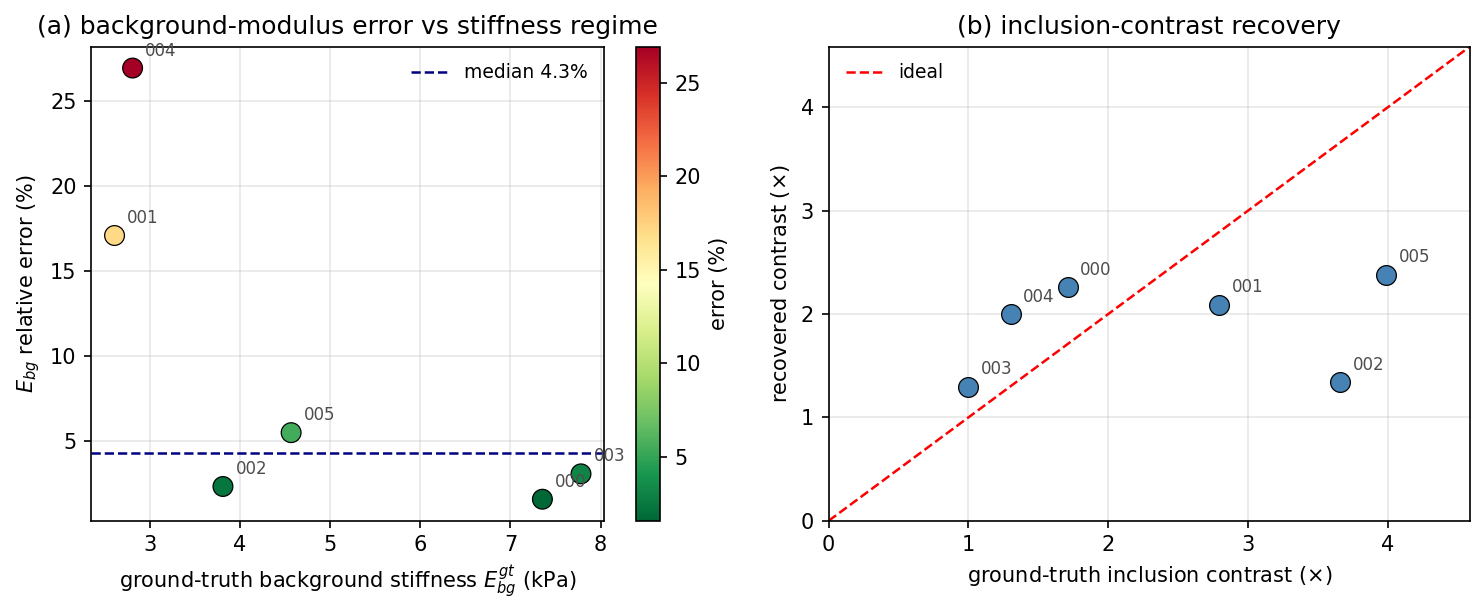
\includegraphics[width=0.85\linewidth]{fig_fem_distribution.png}
\caption{FEM-benchmark inversion across six scenarios. (a) Background-modulus
error vs ground-truth stiffness: accuracy is regime-dependent, degrading on
the two softest backgrounds. (b) Recovered inclusion contrast vs ground
truth (dashed identity).}
\label{fig:fem_dist}
\end{figure}

\paragraph{Force provenance}
\label{sec:force}
We use the empirical error model of an unpublished video-based force
estimator (R3D-18, small-bowel retraction recordings, 6373 samples / 50
recordings: mean absolute error (MAE) 0.295\,N, systematic scale factor
$0.949 \pm 0.140$) and
transport it onto the FEM benchmark. A systematic sweep (force scale
0.80--1.20, recovered $E_{bg}$ ratio 0.846--1.110) follows
Proposition~\ref{prop:forcescale} in direction and is not an exact
one-to-one map, as Remark~\ref{rem:nonlinear} states. With this error
model, the $E_{bg}$ error is 4.1\,$\pm$\,4.0\% and the stiffness contrast
stays within 2.22--2.27$\times$.

\paragraph{Real phantom}
On the \'ETS indentation phantom (6 acquisitions), the image-derived
modulus contrast reaches a median of $3.80\times$ (bootstrap 95\%
confidence interval (CI)
[3.16, 4.34]) against compression-test truth $3.56\times$ (background
$31.0 \pm 1.87$\,kPa, inclusion $8.71 \pm 3.80$\,kPa), a 6.9\% relative
error, stable across 9 sensitivity configurations (3.5--9.3\%). Posterior
intervals contain both ground-truth moduli. The estimate is a contrast, not
an absolute modulus, and Proposition~\ref{prop:forcescale} explains why
this ratio is independent of a global force scale.
Fig.~\ref{fig:ets} shows the per-acquisition estimates.

\begin{figure}[htbp]
\centering
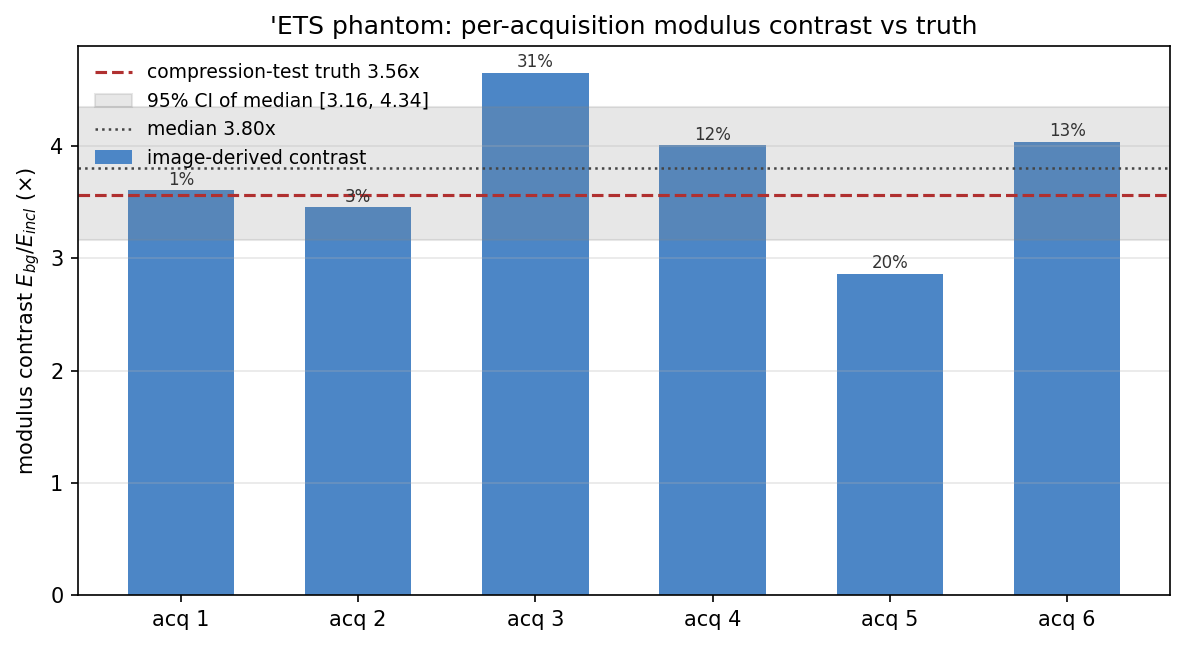
\includegraphics[width=0.7\linewidth]{fig_ets.png}
\caption{\'ETS phantom: per-acquisition image-derived modulus contrast vs
the compression-test truth (dashed), with the bootstrap 95\% CI band and
median. The video-derived contrast is consistent across all six
acquisitions.}
\label{fig:ets}
\end{figure}

\paragraph{Hospital CT geometry construction}
To assess construction of a patient-specific geometry from clinical data,
we reconstruct the liver from an abdominal CT scan of a patient from Henan
Provincial People's Hospital (Fig.~\ref{fig:hospital_ct}). A
right-upper-quadrant liver region is segmented on 82 axial slices and
meshed into a patient-specific liver geometry (178,000 vertices). The CT
provides a patient-specific geometry source; the absolute volume is not
reported because the available slices do not contain spacing metadata.
This CT case is not paired with an endoscopic sequence and therefore does
not validate optical classification or mechanical inversion.

\begin{figure}[htbp]
\centering
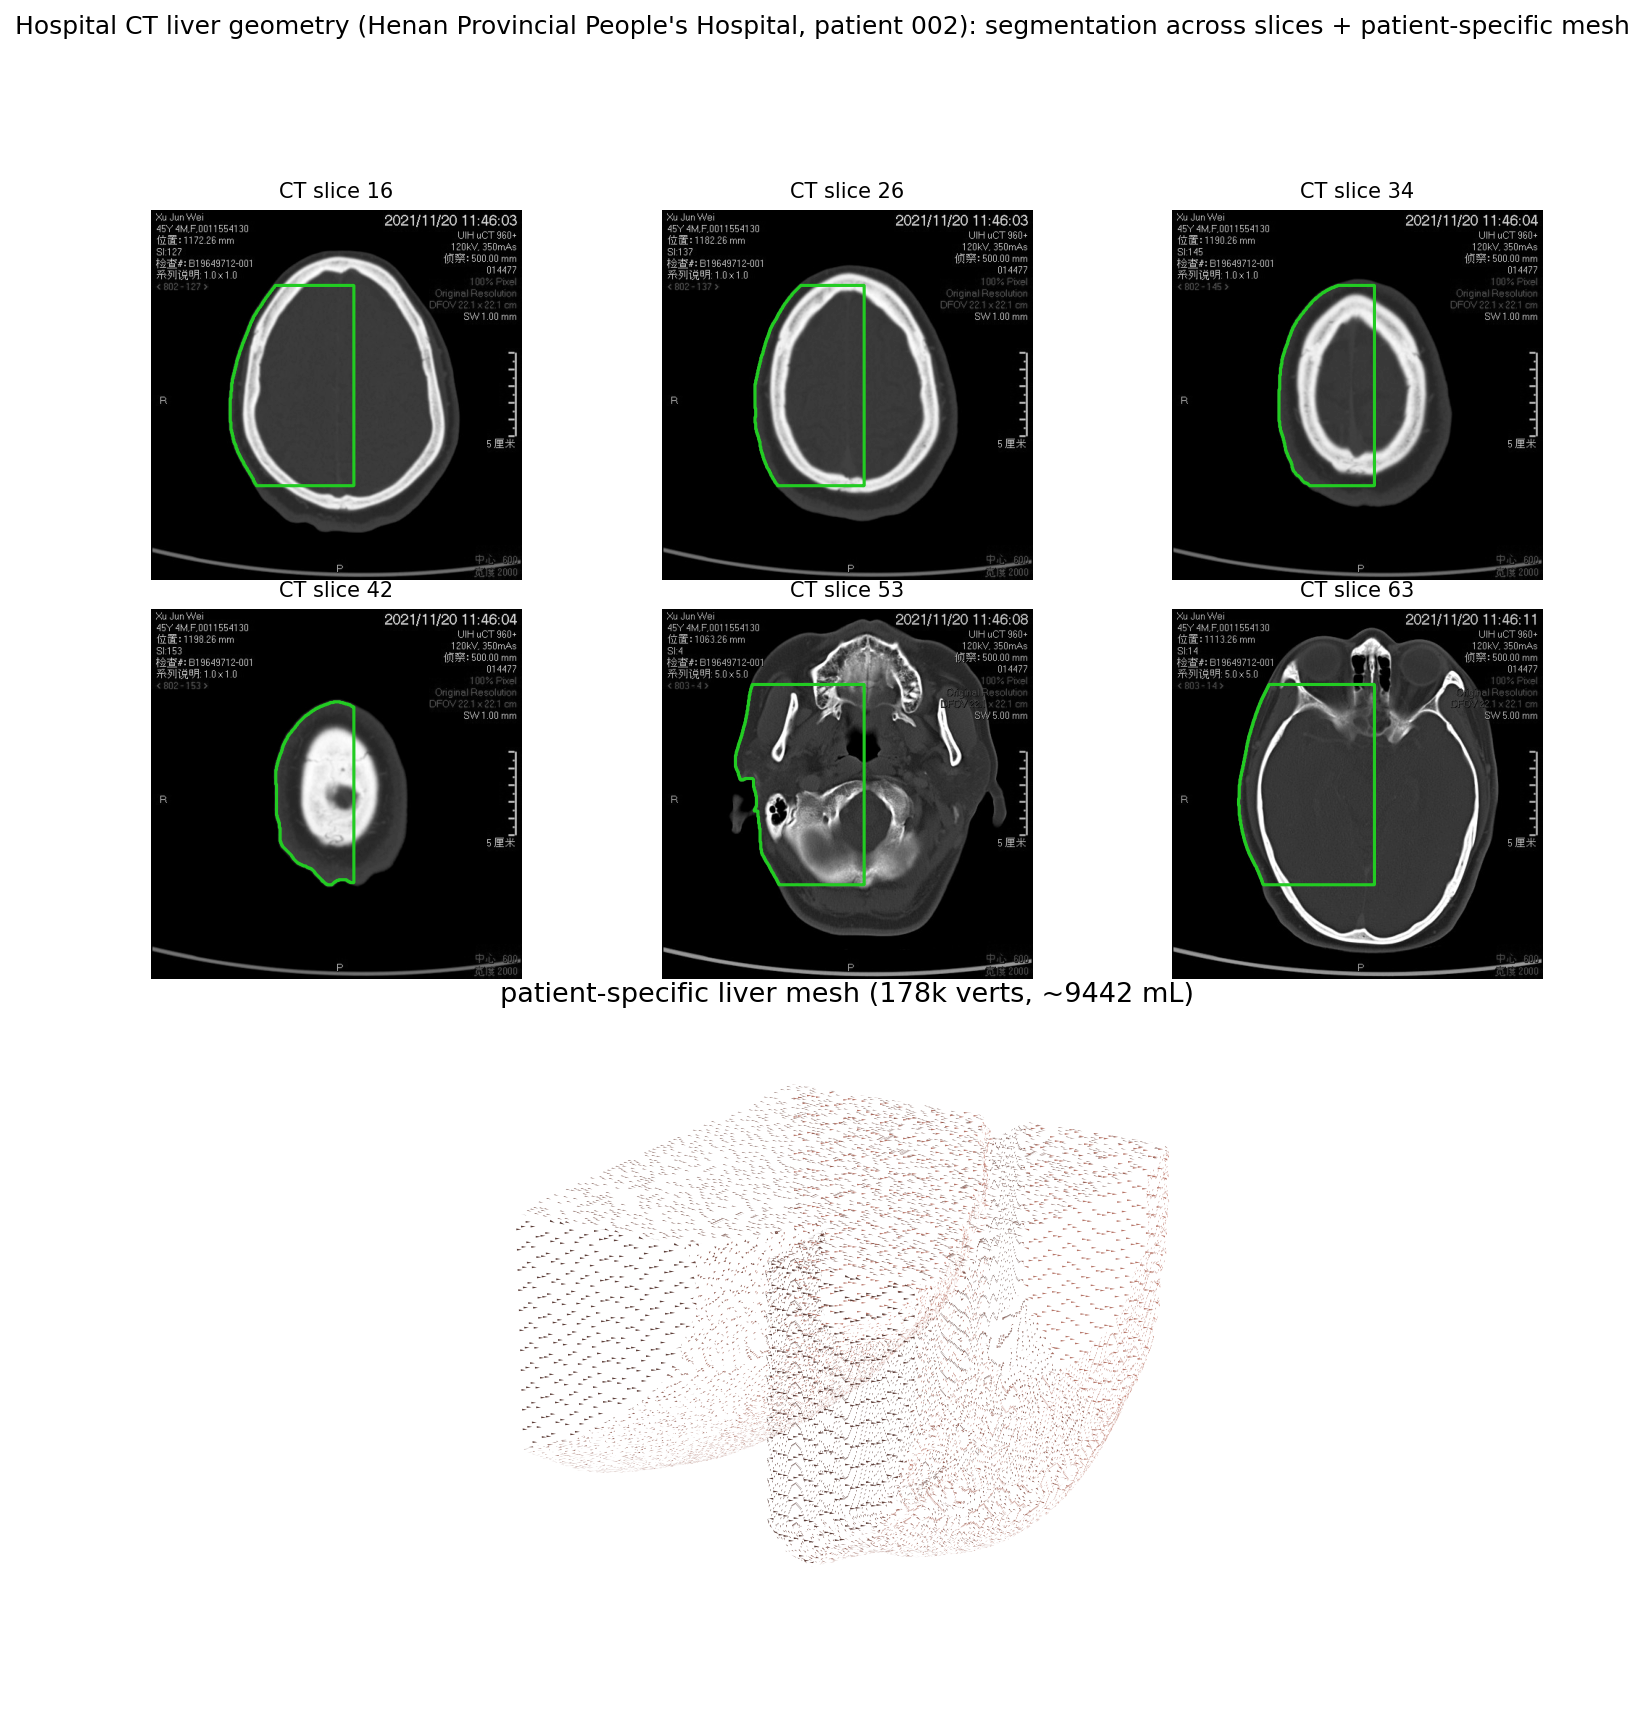
\includegraphics[width=\linewidth]{fig_hospital_ct.png}
\caption{Hospital CT liver geometry (Henan Provincial People's Hospital).
Top two rows: six axial CT slices with the segmented liver region (green).
Bottom: the patient-specific liver mesh reconstructed from the segmentation
(178,000 vertices).}
\label{fig:hospital_ct}
\end{figure}

\begin{figure}[htbp]
\centering
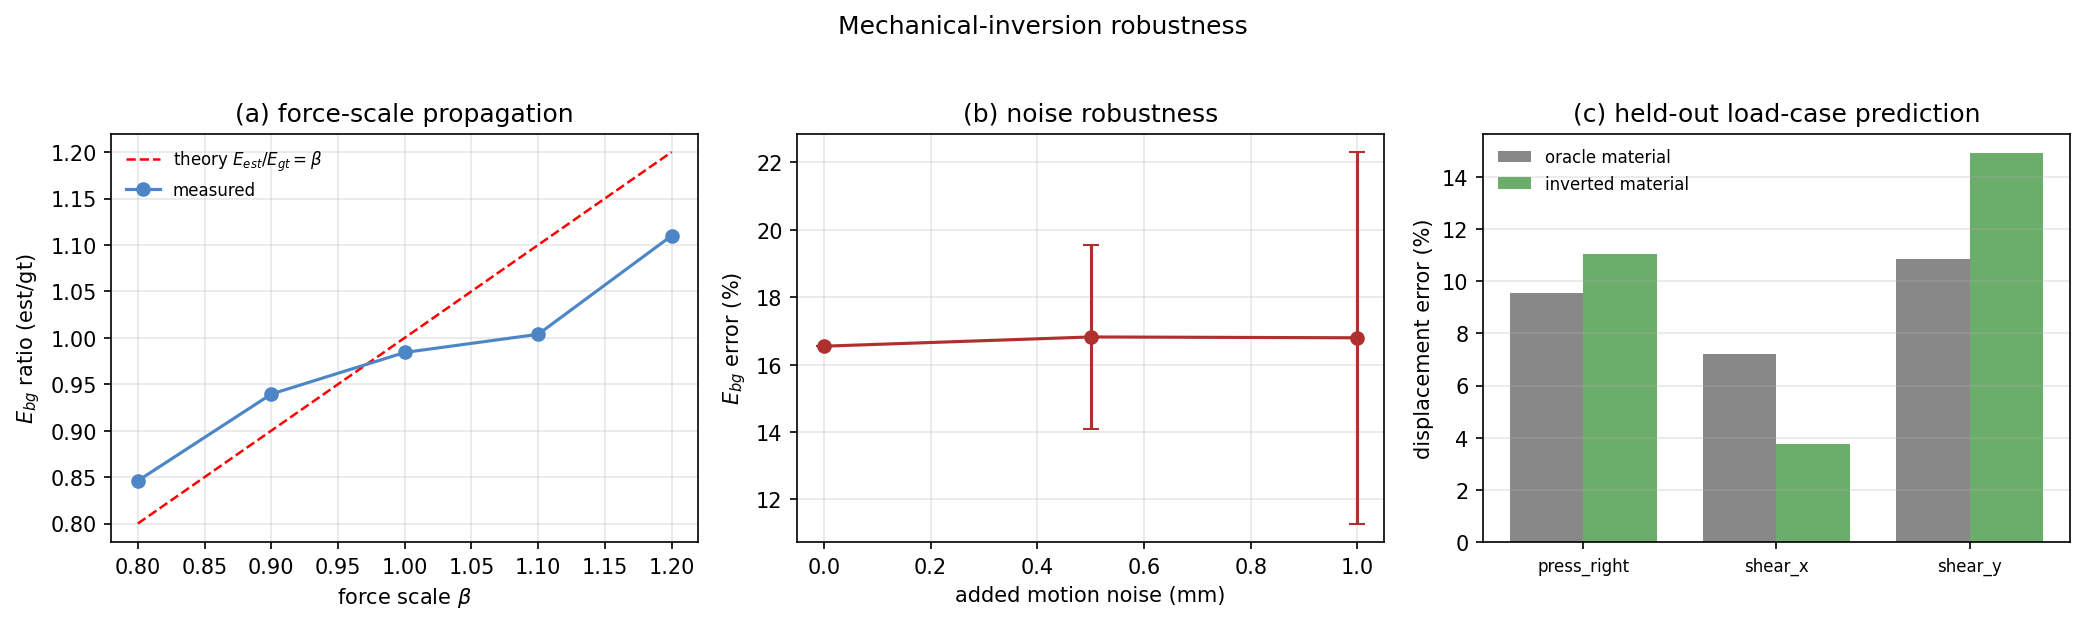
\includegraphics[width=\linewidth]{fig_robustness.png}
\caption{Mechanical-inversion robustness. (a) Force-scale sweep: the
recovered $E_{bg}$ ratio tracks the theoretical one-to-one propagation of
Proposition~\ref{prop:forcescale}. (b) Noise robustness: the $E_{bg}$ error
increases with added motion noise. (c) Held-out load-case
prediction: the inverted material matches the oracle material across three
unseen load cases.}
\label{fig:robustness}
\end{figure}

\paragraph{Mechanics comparison}
Table~\ref{tab:mech_compare} places the mechanical results against the
closest settings in the literature and controlled ablations. Because the
settings differ (known force vs.\ force-free, absolute modulus vs.\
contrast), results are grouped by setting and are not combined into a
single ranking. The audit reports the quantity supported by the available
force and deformation evidence.

\begin{table*}[htbp]
\centering
\caption{Mechanics comparison by setting. Absolute $E$ denotes
absolute-modulus recovery; contrast denotes stiffness-contrast recovery.}
\label{tab:mech_compare}
\small
\begin{tabular}{@{}p{0.20\linewidth}p{0.24\linewidth}p{0.18\linewidth}p{0.24\linewidth}@{}}
\toprule
Method & Setting & Force & Result \\
\midrule
PAC-NeRF \cite{pacnerf} & system identification, multi-view & known & absolute $E$, object-dependent \\
PhysDreamer \cite{physdreamer} & video prior, static & none & relative stiffness only \\
PhysGaussian \cite{physgaussian} & MPM dynamics & manual $E$ & parameters assigned \\
\midrule
Present study (synthetic closed loop) & uniform $E$ & known & absolute $E$: 0.01\% error \\
Present study (FEM benchmark) & two-region, surface-only & measured (5\% error) & absolute $E_{bg}$: median 4.3\% error \\
Present study (force provenance) & two-region & unpublished video estimate & $E_{bg}$: 4.1$\pm$4.0\%; contrast unchanged \\
Present study (real phantom) & strain ratio & none & contrast: 6.9\% error; 95\% CI includes reference \\
\bottomrule
\end{tabular}
\end{table*}

\paragraph{Material recovery}
Beyond geometry and motion, the twin recovers the tissue's optical and
mechanical material. Fig.~\ref{fig:material} shows the recovered albedo and
roughness maps from the canonical field (reconstruction) alongside the mechanical
parameters with their audit tags (inversion): the tissue is classified as liver
(Neo-Hookean), and because no force is instrumented, the Young's modulus,
Poisson ratio, density, viscosity, and friction are tagged
\emph{assumed\_table}, while the optical parameters are \emph{estimated}.

\begin{figure}[htbp]
\centering
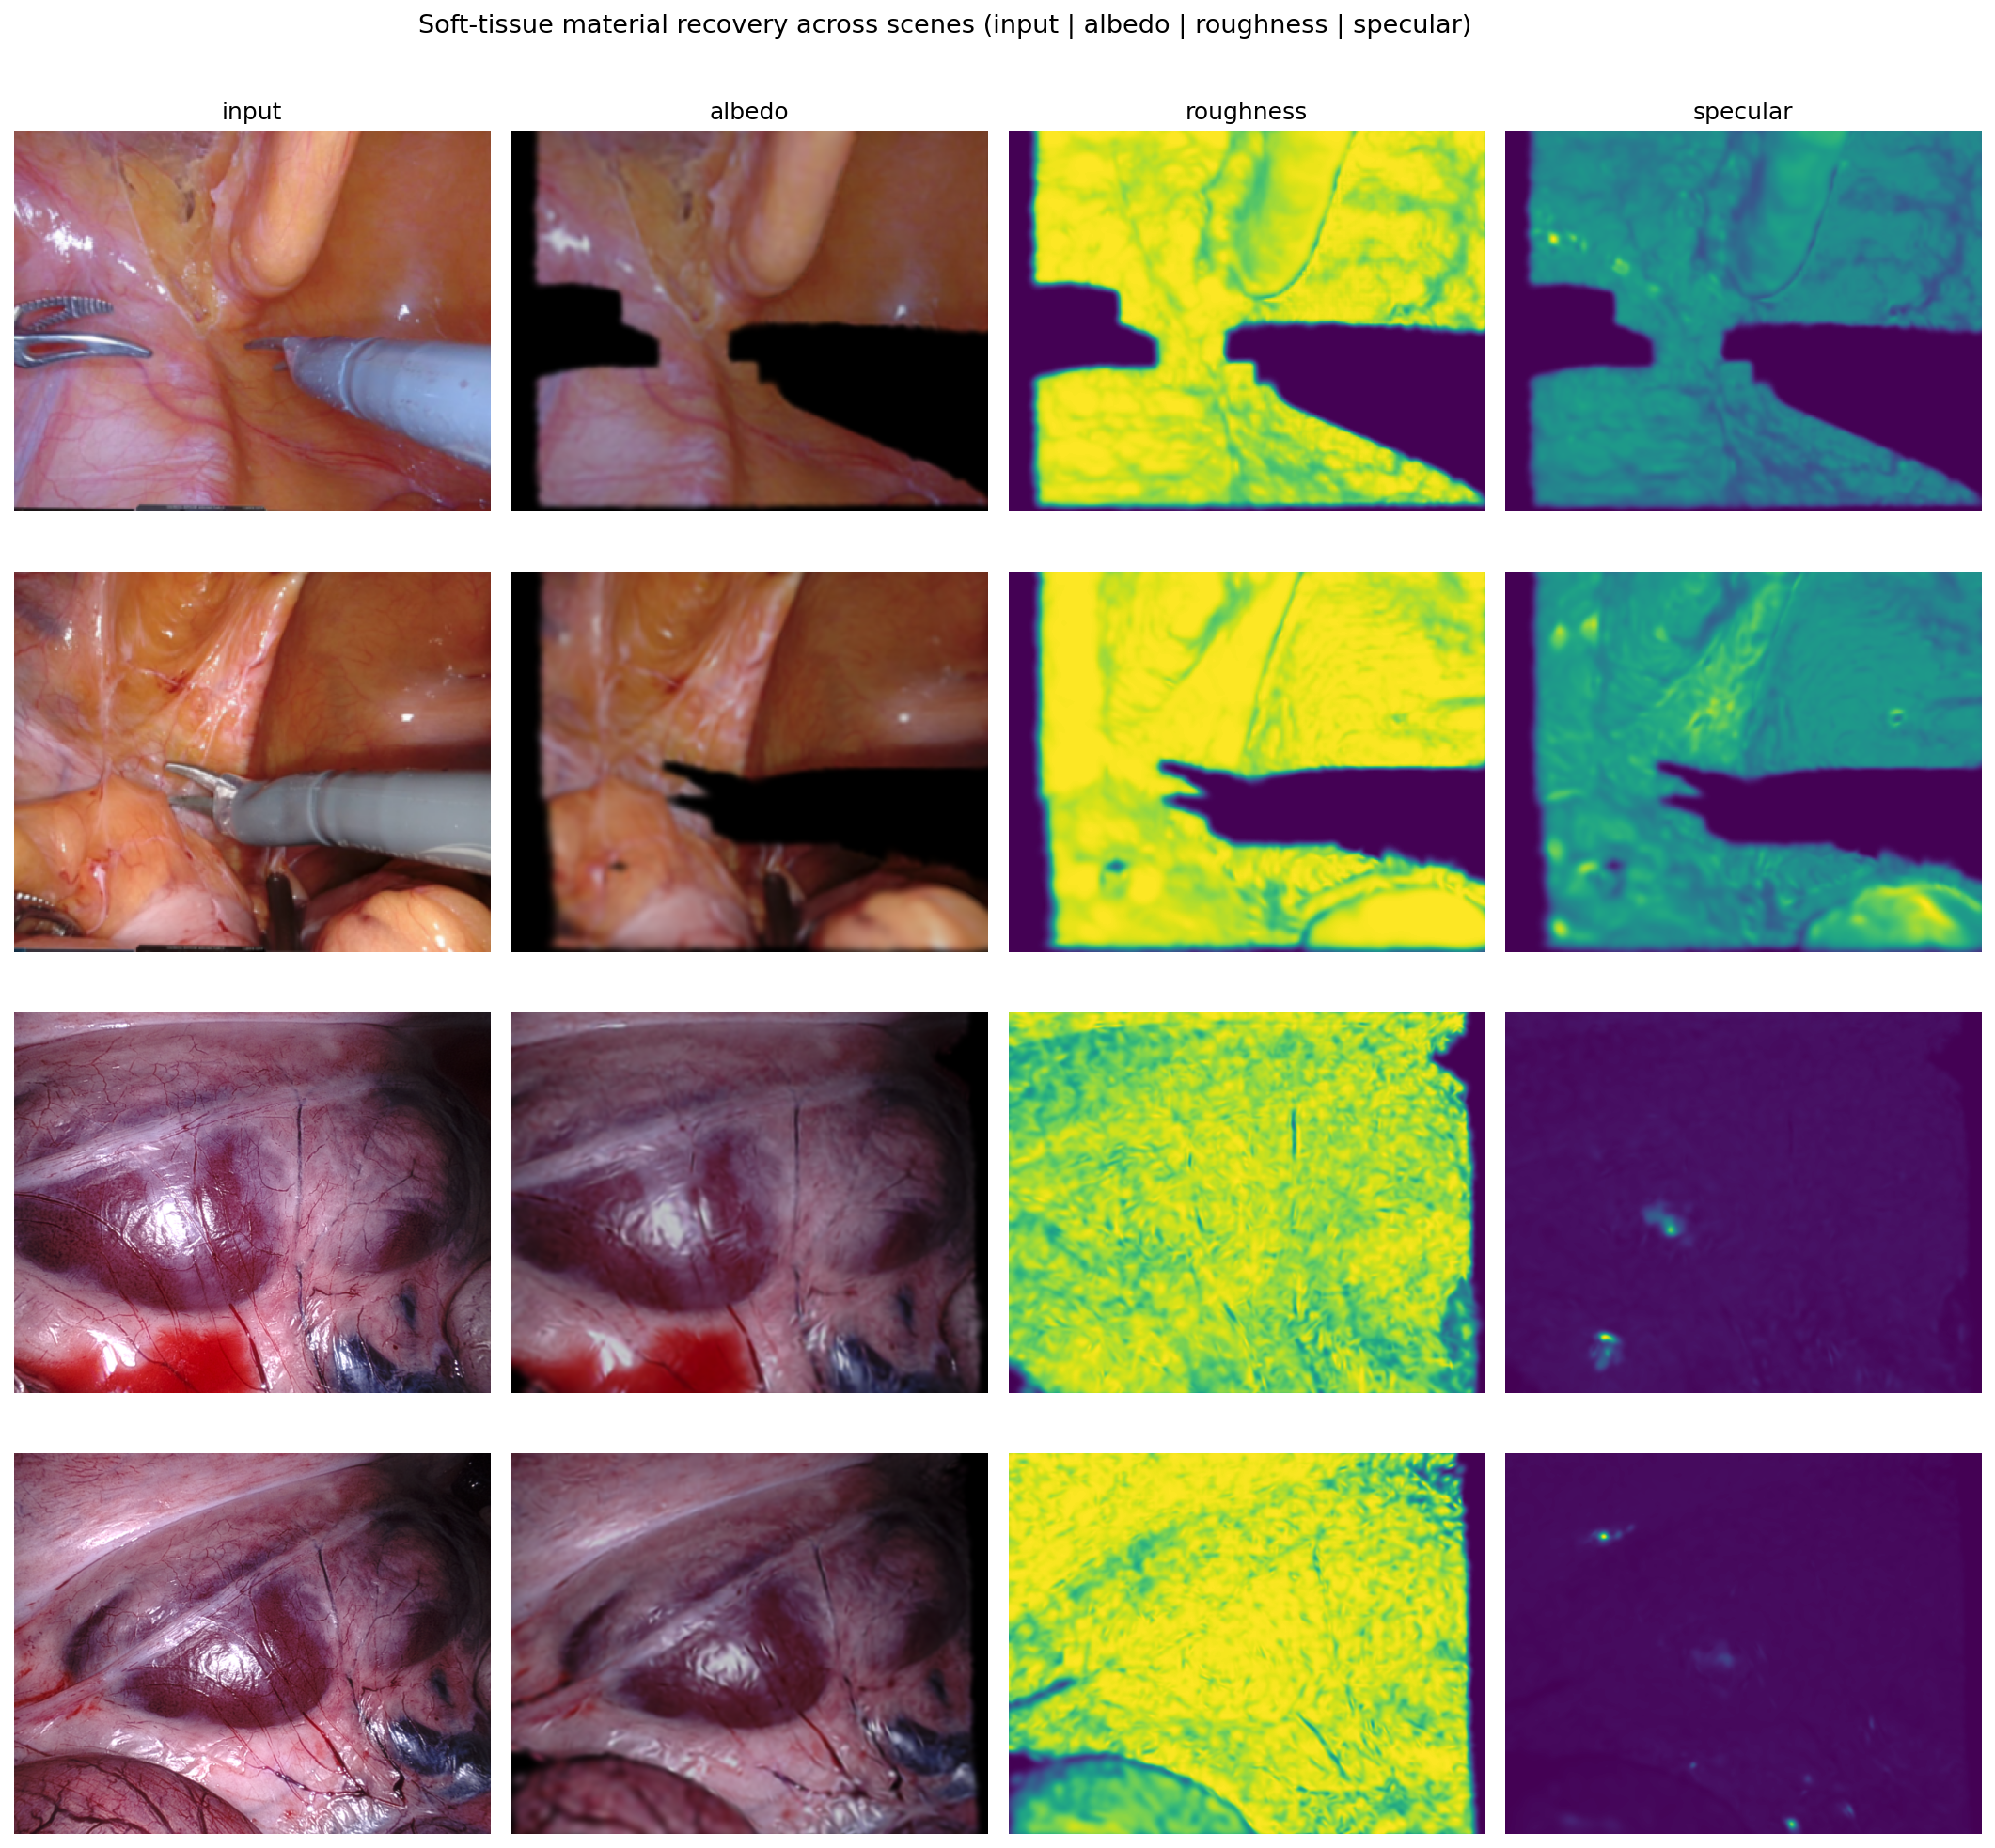
\includegraphics[width=\linewidth]{fig_material_4x4.png}
\caption{Soft-tissue material recovery across four scenes (rows: EndoNeRF
pulling, EndoNeRF cutting, SCARED keyframe\_1, SCARED keyframe\_2).
Columns: input $|$ recovered albedo $|$ recovered roughness $|$ recovered
specular. The optical material is estimated from image observations; the mechanical parameters are
tagged \emph{assumed} (no force instrumented).}
\label{fig:material}
\end{figure}

\subsection{Posterior uncertainty}
\label{sec:uq_exp}
Posterior dispersion was examined as an indicator of parameter
identifiability. The Laplace approximation gives
$\mathrm{std}(\log E_{bg}) = 1.17$
but a much larger $\mathrm{std}(\log E_{incl}) = 21.2$: the data do not
constrain the deep inclusion modulus, consistent with its 30\% estimation
error. The 95\% prediction interval covers 100\% of held-out surface nodes
but is dominated by the unidentified inclusion direction, so the
inclusion modulus is classified as weakly identified.

\subsection{Comparison with related approaches}
\label{sec:comparison}
Table~\ref{tab:position} compares the outputs and assumptions of
representative methods. EndoNeRF, EndoSurf, and EndoGaussian estimate
appearance and geometry but do not provide a mechanical forward operator
$\mathcal{S}$. PhysGaussian requires prescribed material parameters, while
PhysDreamer estimates relative stiffness. PAC-NeRF performs system
identification with known forces and multi-view capture. The present method
combines a simulable representation with explicit parameter provenance and
quantifies the dependence of absolute modulus on force uncertainty.

\subsection{Component-wise comparison}
\label{sec:componentwise}
The reconstruction, tracking, and inversion results use different
protocols from the corresponding published methods. Table~\ref{tab:componentwise}
therefore reports component-level context rather than an end-to-end
ranking. Reconstruction is related to endoscopic novel-view synthesis,
whereas mechanical inversion is related to physics-based system
identification. No direct reference protocol was identified for the
parameter-provenance map.

\begin{table*}[htbp]
\centering
\caption{Component-level context. Results obtained under different
protocols are not interpreted as a ranking.}
\label{tab:componentwise}
\footnotesize
\begin{tabular}{@{}p{0.14\linewidth}p{0.22\linewidth}p{0.22\linewidth}p{0.22\linewidth}@{}}
\toprule
Component & Reference method & Reference result & Present study \\
\midrule
Reconstruction & EndoGaussian \cite{endogaussian} (NVS) & NVS protocol, not re-run & 36.79\,dB (canonical, tissue-masked) \\
Deformation tracking & DefSLAM \cite{defslam} & monocular deforming tracking & fixed topology with rollback; no divergence \\
Mechanics (absolute $E$) & PAC-NeRF \cite{pacnerf} & object-dependent, known force & median 4.3\% error (measured force) \\
Mechanics (contrast) & PhysDreamer \cite{physdreamer} & relative only & contrast 6.9\% error with CI (phantom) \\
Provenance audit & none & not available & measured / estimated / assumed \\
\bottomrule
\end{tabular}
\end{table*}

The reconstruction values are canonical, tissue-masked fits and are not
directly comparable with held-out novel-view metrics. The tracking and
mask comparisons are controlled ablations on the same data. The 4.3\%
FEM median is calculated on six selected scenarios and is not an estimate
over the full 60-scenario benchmark. Figure~\ref{fig:taskcmp} and
Table~\ref{tab:taskcmp} distinguish matched from unmatched protocols.

\begin{figure}[htbp]
\centering
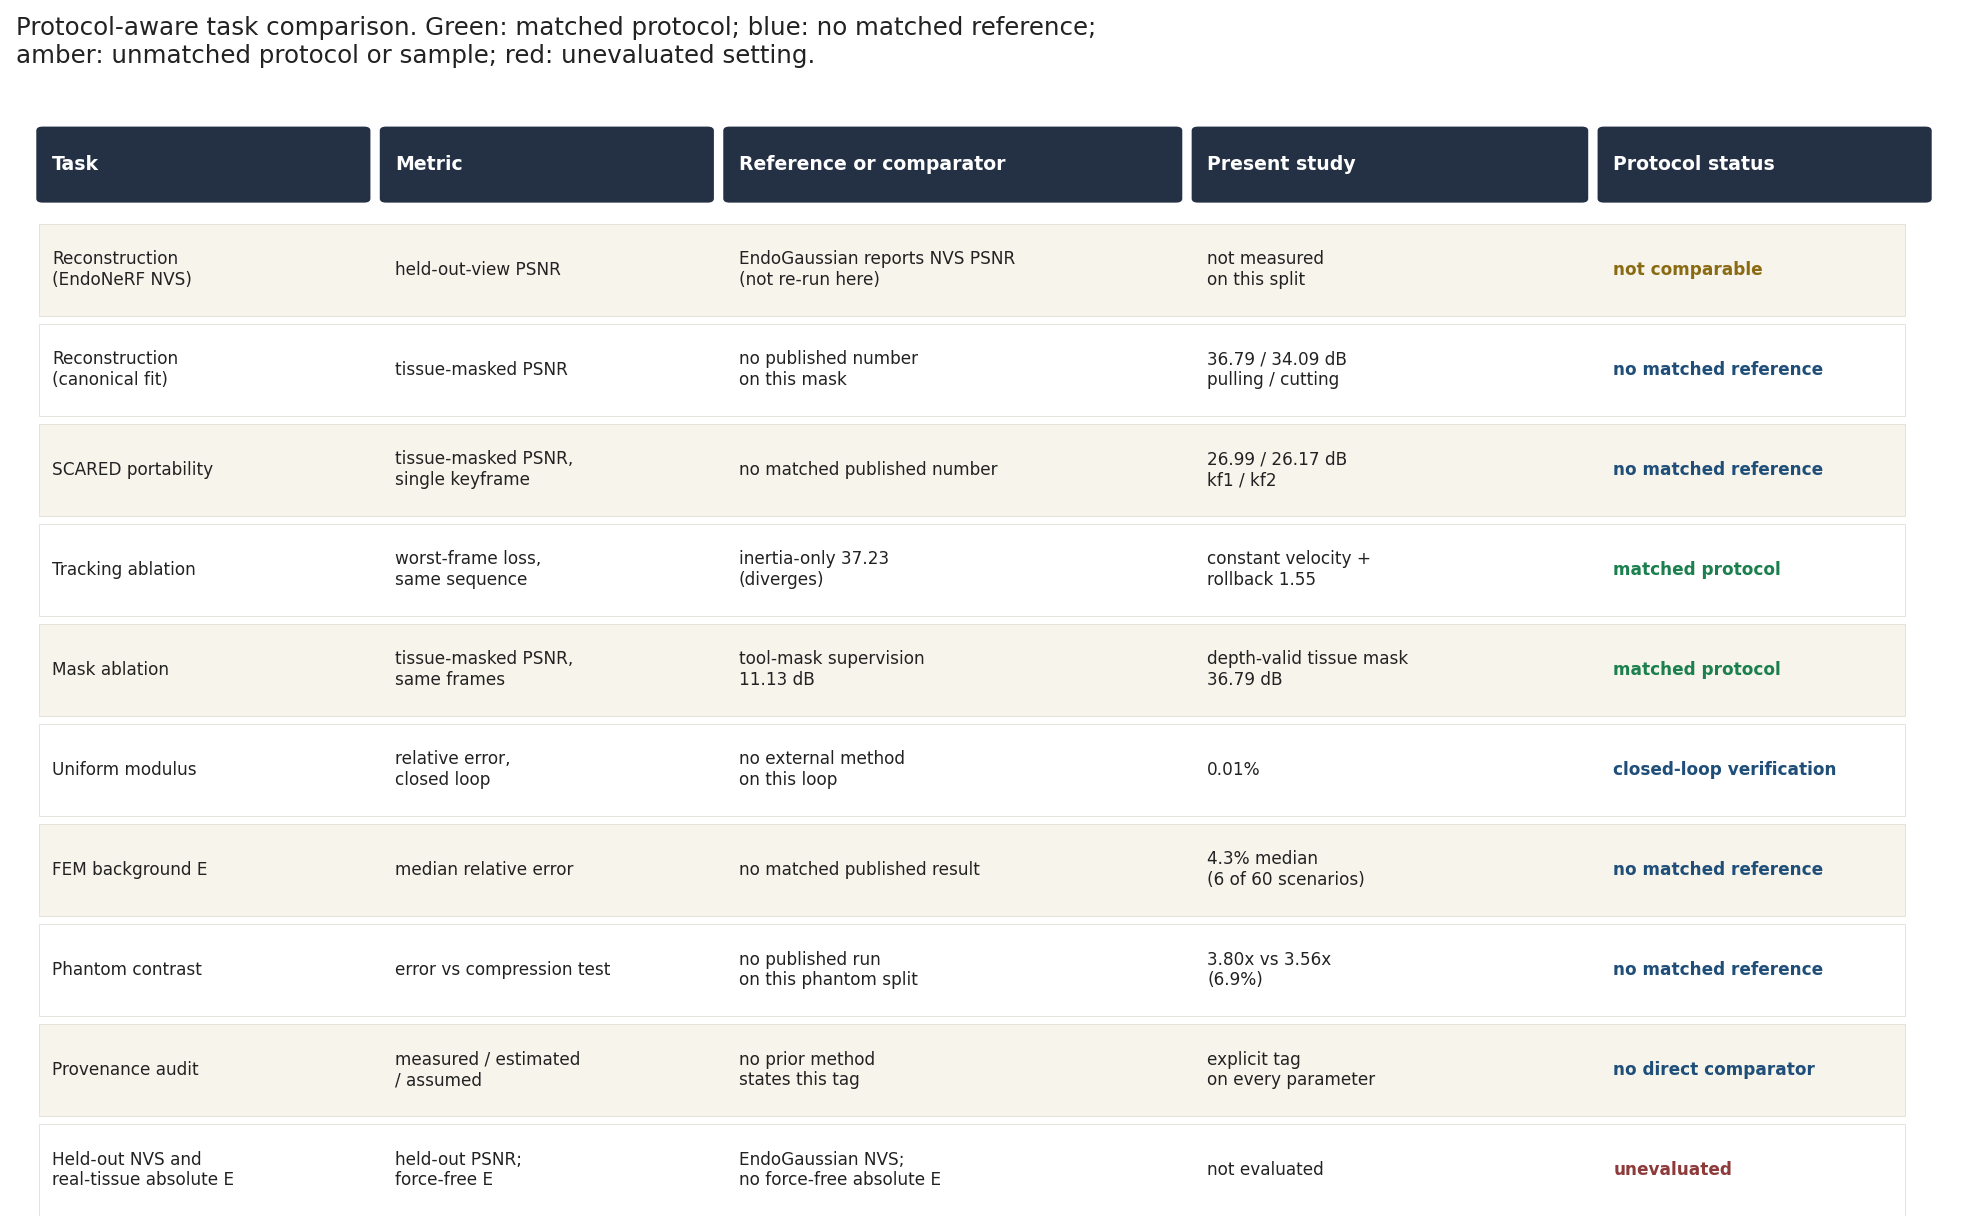
\includegraphics[width=\linewidth]{fig_task_comparison.png}
\caption{Protocol-aware task comparison. Green denotes a matched-protocol
ablation; blue denotes a result without a matched published value; amber
denotes an unmatched protocol; and red denotes an unevaluated setting.}
\label{fig:taskcmp}
\end{figure}

\begin{table*}[htbp]
\centering
\caption{Protocol-aware summary. Values from different protocols are
included for context and are not compared quantitatively.}
\label{tab:taskcmp}
\footnotesize
\begin{tabular}{@{}p{0.15\linewidth}p{0.13\linewidth}p{0.19\linewidth}p{0.18\linewidth}p{0.13\linewidth}@{}}
\toprule
Task & Metric & Reference value & Present study & Protocol relation \\
\midrule
EndoNeRF novel views & held-out PSNR & EndoGaussian, NVS, not re-run & not measured & different protocol \\
Canonical fit & tissue-masked PSNR & none on this mask & 36.79 / 34.09\,dB & reported \\
SCARED keyframes 1--2 & tissue-masked PSNR & none matched & 26.99 / 26.17\,dB & reported \\
Tracking & worst-frame loss & inertia-only 37.23 & 1.55 & same protocol \\
Tissue mask & tissue-masked PSNR & tool mask 11.13\,dB & 36.79\,dB & same protocol \\
Uniform modulus & relative error & none on this loop & 0.01\% & closed loop \\
FEM $E_{bg}$ & median relative error & no matched published result & 4.3\% on 6 scenes & reported \\
Phantom contrast & comparison with compression test & none on this split & 6.9\% & reported \\
Absolute $E$, real endoscopy, no force & relative error & not available & not evaluated & unevaluated \\
\bottomrule
\end{tabular}
\end{table*}

\subsection{Ablations}
\begin{table}[htbp]
\centering
\caption{Ablations.}
\label{tab:ablation}
\footnotesize
\begin{tabular}{lll}
\toprule
Ablation & Variant & Metric \\
\midrule
Mask supervision & instrument mask & 11.13\,dB \\
Mask supervision & depth-valid tissue mask & \textbf{36.79\,dB} \\
Number of Gaussians & 4000 / 6498 / 10000 & 35.31 / 36.86 / \textbf{38.21}\,dB \\
Temporal-model & inertia-only & 37.23 (divergence) \\
Temporal-model & constant velocity + rollback & \textbf{1.55} \\
Parameterization & per-node field & contrast $1.69\times$ \\
Parameterization & two-region & \textbf{$3.19\times$} \\
Forward model & mass--spring surrogate & contrast $4.19\times$ (true $1.71\times$) \\
Forward model & FEM-in-the-loop & \textbf{$2.26\times$} (true $1.71\times$) \\
\bottomrule
\end{tabular}
\end{table}

The same Gaussians are used for rendering and deformation tracking on the
endoscopic sequences; their displacements support regional contrast
estimation. On the separate force-calibrated FEM benchmark, background
modulus has a median error of 4.3\% when the force is measured, and
4.1\,$\pm$\,4.0\% when the force comes from the unpublished video
estimator. The stiffness contrast stays within 2.22--2.27$\times$. When no
force is available, the reported quantity is stiffness contrast (6.9\%
error, interval covering the compression-test value), in agreement with
Proposition~\ref{prop:forcescale}. The Laplace posterior marks the
inclusion modulus as unidentified, and parameters copied from the tissue
table are tagged assumed.

%% ===================================================================
\section{Discussion}
\label{sec:discussion}
%% ===================================================================

Geometry and reflectance are constrained directly by image and depth
observations. In contrast, Young's modulus is identifiable only when both
deformation and loading are available. The force-provenance analysis
(Sec.~\ref{sec:force}) confirms that uncertainty in the force scale
propagates to absolute modulus but largely cancels in regional stiffness
contrast. Absolute modulus and stiffness contrast should therefore be
interpreted separately.

\paragraph{Example provenance record}
For the pulling sequence, albedo and roughness are marked estimated because
they are fitted to image observations. Tissue class is also marked estimated
because it is selected by an optical heuristic. Young's modulus is marked
assumed (liver prior: median 6\,kPa; 95\% interval 2.3--16.0\,kPa) because
no force was instrumented. Regional stiffness contrast is marked estimated
from deformation, while Poisson's ratio and viscosity retain their
table-derived assumed labels. Simulations based on this sequence should
therefore propagate the prior interval rather than use a single absolute
modulus.

The proposed representation could support simulation of alternative
instrument loads after reconstruction from an intra-operative video.
However, the present evidence establishes technical feasibility rather
than clinical utility. Force-instrumented tissue experiments, prospective
patient data, and task-specific validation are required before the method
can be considered for surgical decision support. Elastography provides the
closest clinical analogue because it also estimates stiffness contrast
from induced deformation \cite{ophir1991}. The phantom experiment indicates
agreement with independent compression testing for this relative
quantity; it does not establish equivalence with clinical elastography.

Any future clinical implementation would also require institutional data
governance, calibrated confidence thresholds, and regulatory evaluation.
The provenance map provides a technical mechanism for exposing the
evidence associated with each parameter, but does not by itself establish
clinical safety.

\paragraph{Reproducibility}\label{sec:repro}
Source code, evaluation scripts, and data-split definitions are available
in the project repository. Every numerical result
reported in this paper is produced by the released end-to-end scripts,
which cover reconstruction, tracking, and inversion on EndoNeRF and SCARED, the FEM
benchmark inversion, the force-provenance analysis, and the phantom audit;
each script writes a machine-readable summary and the corresponding
figures, from which every number in the paper is drawn.

\subsection{Limitations}
\label{sec:threats}
The reconstruction values are tissue-masked fits and cannot be compared
directly with held-out, full-image novel-view metrics. The principal FEM
analysis uses six selected scenarios from a synthetic 60-scenario
benchmark; the observed dependence on background stiffness is therefore
descriptive rather than a population-level estimate. The force estimator
and its empirical error model are unpublished and have not been
independently validated. The \'ETS phantom uses ultrasound rather than
endoscopic colour images, so it validates mechanical contrast but not the optical
reconstruction. The mass--spring surrogate has an 82\% forward error and is
not used to support absolute mechanical estimates on real data. In
addition, the clinical CT experiment contains one de-identified case and
validates geometry construction only. These limitations preclude claims of
clinical performance or absolute-modulus recovery from uninstrumented
endoscopic video.

%% ===================================================================
\section{Methods}
\label{sec:method}
%% ===================================================================

\begin{figure*}[htbp]
\centering
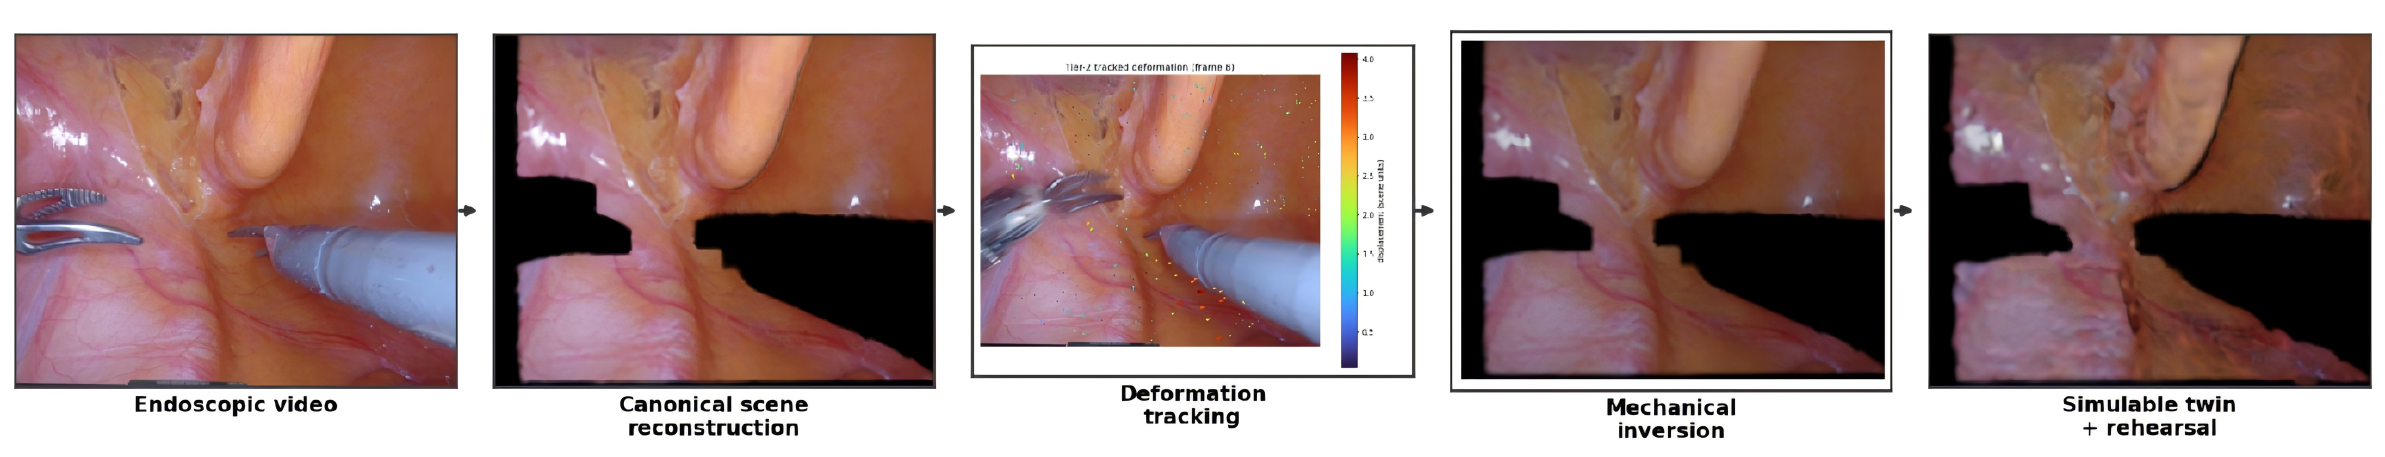
\includegraphics[width=\textwidth]{fig_architecture_results.png}
\caption{Model architecture and representative outputs. The endoscopic
video is reconstructed as a canonical Gaussian field and tracked with
fixed primitive identities. Tracked surface displacement supports relative
stiffness estimation on uninstrumented video and provides the observation
interface for known-force mechanical inversion. The provenance map records
the evidential status of each parameter.}
\label{fig:architecture}
\end{figure*}

The study was designed as a computational methods investigation of whether
a monocular endoscopic reconstruction can be extended to a mechanically
simulable representation with explicit parameter provenance. Evaluation
combines public endoscopic and phantom data, a synthetic FEM benchmark,
and one de-identified clinical CT case. The following subsections define
the representation, reconstruction, deformation tracking, mechanical
inversion, force-scale analysis, and provenance map.

\subsection{Study design and data sources}
\label{sec:setup}

\paragraph{Datasets.}
Table~\ref{tab:datasets} summarizes the five data sources and their roles.

\begin{table*}[htbp]
\centering
\caption{Data sources. ``GT'' indicates the ground truth used for evaluation.}
\label{tab:datasets}
\scriptsize
\begin{tabular}{@{}p{0.14\linewidth}p{0.17\linewidth}p{0.11\linewidth}p{0.17\linewidth}p{0.17\linewidth}@{}}
\toprule
Dataset & Modality & Scale & GT used & Used for \\
\midrule
EndoNeRF (2 scenes) & monocular video, depth, instrument masks & 63 / 156 frames & depth, instrument masks & reconstruction and tracking \\
SCARED & stereo laparoscopy + metric depth & 2 keyframes & metric depth (mm) & reconstruction (portability) \\
FEM benchmark & synthetic FEM (Neo-Hookean tetrahedra) & 60 scenarios, 4 loads & $E_{bg}$, $E_{incl}$, forces & mechanical inversion (closed loop) \\
\'ETS phantom & ultrasound + force & 6 acquisitions & compression-test $E$ & mechanical inversion (real phantom) \\
Hospital CT & abdominal CT (1 patient) & 82 slices & CT anatomy & geometry construction \\
\bottomrule
\end{tabular}
\end{table*}

EndoNeRF frames are loaded at $0.5\times$ scale, with depth used both for
the canonical point cloud and for the tissue mask $\Omega$ of
\eqref{eq:mask} \cite{endonerf}; SCARED keyframes at $0.5\times$ scale with intrinsics from
the calibration file \cite{scared}; the FEM benchmark is used with the measured (not
true) forces and the noisy (not true) surface motion as inversion inputs;
the first six FEM scenario directories in lexical order are used for the
main inversion, providing deterministic selection independent of
performance; and the \'ETS phantom is used at the frame level with
synchronized force \cite{etsphantom}.

\paragraph{Evaluation metrics.}
Reconstruction quality is reported as tissue-masked PSNR on
$\Omega$ (all-image metrics are lower by design because tools are masked
out). Tracking quality is measured by the per-frame and worst-frame
photometric loss. Mechanical accuracy is measured by (i) the relative error
of the recovered modulus, $|E^{est} - E^{gt}| / E^{gt}$; (ii) the
inclusion-contrast ratio $E_{incl}/E_{bg}$ against ground truth; (iii) the
held-out load-case displacement error
$\|u(E^{est}) - u^{obs}\| / \mathrm{mean}\|u^{obs}\|$; and (iv) the 95\%
prediction-interval coverage of held-out surface nodes.

\paragraph{Comparison methods.}
For reconstruction we compare against the published novel-view-synthesis
numbers of EndoNeRF \cite{endonerf}, EndoSurf \cite{endosurf}, and
EndoGaussian \cite{endogaussian}, noting that these use a different
protocol (held-out views, full image) and are therefore indicative rather
than strictly comparable (Table~\ref{tab:recon_compare}). For mechanics we
compare against the system-identification setting of PAC-NeRF
\cite{pacnerf}, the relative-stiffness setting of PhysDreamer
\cite{physdreamer}, and controlled ablations (per-node field versus
two-region, mass--spring surrogate versus FEM-in-the-loop).

\paragraph{Implementation.}
Reconstruction uses 800--1000 Adam iterations and approximately
6.5--7.7 thousand Gaussians on an RTX 5090 with the gsplat backend
(${\sim}21$\,s per scene). Tracking uses 40--50 iterations per frame, and
mechanical inversion uses 200--400 iterations. The six-scenario FEM sweep
requires approximately 80\,min.

\paragraph{Statistical analysis.}
Results are summarized with per-scene values, means, medians, and relative
errors as specified for each experiment. The phantom median is accompanied
by a nonparametric bootstrap 95\% confidence interval. No hypothesis tests
or power calculations were performed because the experiments evaluate
algorithmic accuracy on fixed benchmark cases rather than estimate a
clinical population effect. All reported values are generated by the
released scripts (Sec.~\ref{sec:repro}).

\subsection{Soft-tissue digital twin}
\label{sec:twin}
\begin{definition}[Soft-tissue digital twin]
\label{def:twin}
A soft-tissue digital twin is a tuple
$\mathcal{T} = (G, \{\Delta_t\}, \Theta, \mathcal{A})$, where $G$ is a
canonical geometric and optical scene representation, $\{\Delta_t\}$ is a
deformation sequence on $G$, $\Theta$ is a set of physical parameters
(elastic, viscous, inertial, optical), and $\mathcal{A}$ is an audit map
assigning to each $\theta \in \Theta$ a provenance tag and confidence. The
twin is \emph{simulable} if there exists a forward operator
$\mathcal{S} : (G, \Theta, f) \mapsto u$ mapping a load $f$ to a
deformation $u$, and it is \emph{audited} if $\mathcal{A}$ is complete
(every $\theta$ is tagged).
\end{definition}

The input is a sequence of endoscopic frames
$\{I_t\}_{t=1}^{T}$ with per-frame depth maps $D_t$ and tool masks $M_t$;
the output is the twin $\mathcal{T}$. As shown in
Fig.~\ref{fig:architecture}, the canonical Gaussian field $G$ is
reconstructed, displaced while preserving primitive identity, and coupled
to a mechanical forward operator. The audit map is attached to the
resulting parameters. Figure~\ref{fig:twin_complete} illustrates the
result on an endoscopic sequence, and Table~\ref{tab:notation} defines the
notation.

\begin{table}[htbp]
\centering
\caption{Main symbols.}
\label{tab:notation}
\small
\begin{tabular}{@{}p{0.28\linewidth}p{0.64\linewidth}@{}}
\toprule
Symbol & Meaning \\
\midrule
$I_t, D_t, M_t$ & frame image, depth map, tool mask \\
$G=\{g_i\}_{i=1}^{N}$ & canonical Gaussian field, $N$ primitives \\
$\mathbf{x}_i, \Sigma_i, o_i, \mathbf{n}_i$ & position, covariance, opacity, normal of $g_i$ \\
$\rho_d,\rho_s,\alpha,m,a$ & diffuse, specular, roughness, metalness, absorption \\
$\Delta_t$ & per-Gaussian displacement at frame $t$ \\
$E, \nu$ & Young's modulus (Pa), Poisson ratio \\
$u, f$ & nodal displacement, external force \\
$E_{bg}, E_{incl}$ & background and inclusion modulus \\
$q_i, Q(q_i), s_i$ & rotation quaternion, its rotation matrix, and scale of $g_i$ \\
$c_i, \alpha_i$ & shaded color and projected opacity of $g_i$ \\
$E_d, D, G_s, F$ & diffuse irradiance, GGX distribution, Smith geometry, Fresnel \\
$\mathbf{l}, \mathbf{v}$ & light direction and view direction \\
$\Omega, \epsilon$ & tissue pixels, depth-validity threshold \\
$\Gamma_{obs}$ & observed surface nodes used for inversion \\
$C_r, d_r, \kappa_r$ & spatial region, mean displacement, relative stiffness \\
$\epsilon_d$ & displacement stabilizer in the contrast estimate \\
$\lambda_{ph},\lambda_d,\lambda_\alpha$ & photometric, depth, and alpha loss weights \\
$\lambda_s,\lambda_a$ & spatial smoothness and acceleration weights \\
$\mathcal{N}(i)$ & $k$ nearest neighbors of Gaussian $i$ \\
$R, f_{int}, f$ & equilibrium residual, internal force, applied force \\
$\gamma, \mathcal{R}$ & regularization weight and regularizer \\
$F, J$ & deformation gradient and $J=\det F$ \\
$\mu, \lambda$ & Lam\'e parameters at fixed $\nu$ \\
$\beta$ & global force or modulus scale \\
$K, \tilde{K}$ & stiffness matrix and its modulus-free factor \\
$\hat{f}, g_\phi, \phi$ & estimated force, force network, backbone feature \\
$\tau(\theta), c(\theta)$ & provenance tag and confidence of parameter $\theta$ \\
\bottomrule
\end{tabular}
\end{table}

\subsection{Canonical scene reconstruction}
\label{sec:tier1}
Reconstruction builds $G$. Each Gaussian $g_i$ stores a position
$\mathbf{x}_i \in \mathbb{R}^3$, an anisotropic covariance
$\Sigma_i = Q(q_i)\,\mathrm{diag}(s_i^2)\,Q(q_i)^{\top}$ with rotation
quaternion $q_i$ and scale $s_i$, an opacity $o_i \in [0,1]$, a unit normal
$\mathbf{n}_i$, and BRDF parameters $(\rho_d, \rho_s, \alpha, m, a)$. A
softmax energy budget enforces a partition of unity,
\begin{equation}
\rho_d + \rho_s + a = 1, \qquad \rho_d,\rho_s,a \ge 0,
\label{eq:budget}
\end{equation}
so that no primitive reflects more energy than it receives. Images are
formed by front-to-back alpha compositing,
\begin{equation}
\hat{I} = \sum_{i=1}^{N} c_i\,\alpha_i \prod_{j<i}(1-\alpha_j),
\label{eq:render}
\end{equation}
where $c_i$ is the shaded color of $g_i$ and $\alpha_i$ its projected
opacity. The shaded color follows a Cook--Torrance microfacet BRDF
\cite{cooktorrance} split into a diffuse and a specular lobe,
\begin{equation}
c_i = \underbrace{\frac{\rho_d}{\pi}\,E_d}_{\text{diffuse}}
+ \underbrace{\rho_s\,\frac{D(\alpha)\,G_s\,F}{4\,(\mathbf{n}\cdot\mathbf{l})(\mathbf{n}\cdot\mathbf{v})}}_{\text{specular}},
\label{eq:cooktorrance}
\end{equation}
where $E_d$ is the diffuse irradiance, $D(\alpha)$ the GGX normal
distribution, $G_s$ the Smith geometry term, $F$ the Schlick Fresnel term,
$\mathbf{l}$ the light direction, and $\mathbf{v}$ the view direction. The
highlight-free diffuse image is obtained by setting the specular lobe to
zero.

A key endoscopic adaptation concerns the supervision mask. The EndoNeRF
\texttt{masks/} channel marks \emph{tools}, not tissue, and tools have no
valid depth. We therefore define the tissue pixel set as
\begin{equation}
\Omega = \{(u,v) : D(u,v) > \epsilon \} \setminus M,
\label{eq:mask}
\end{equation}
with $\epsilon$ a small depth-validity threshold, and supervise only on
$\Omega$. Supervising on the tool mask instead of $\Omega$ degrades
reconstruction by ${\sim}25$\,dB (Table~\ref{tab:ablation}). The reconstruction
objective is
\begin{equation}
\mathcal{L}_1 = \lambda_{ph}\,\mathcal{L}_{photo} + \lambda_d\,\mathcal{L}_{depth} + \lambda_\alpha\,\mathcal{L}_{\alpha},
\label{eq:tier1loss}
\end{equation}
with non-negative weights $\lambda_{ph},\lambda_d,\lambda_\alpha$, a masked
$L_1 + 0.5\,L_2$ photometric term $\mathcal{L}_{photo}$ on $\Omega$, a
depth $L_1$ term $\mathcal{L}_{depth}$ on $\Omega$, and an alpha
binary-cross-entropy term
$\mathcal{L}_{\alpha}$ toward the tissue mask. Lighting is an
endoscope-co-located directional light plus a strong ambient
spherical-harmonic lobe, so appearance approximates albedo; a learnable
exposure closes the residual gap.

\subsection{Deformation tracking}
\label{sec:tier2}
Tracking estimates $\{\Delta_t\}$ as a per-Gaussian displacement
$\Delta_t \in \mathbb{R}^{N \times 3}$ on the canonical topology, keeping
correspondences fixed across time. Fixed correspondence is what
distinguishes a twin from a per-frame rebuild: the same primitive is
followed through time, so its trajectory is a boundary condition. Naive
inertia-only tracking (penalizing $\|\Delta_t - \Delta_{t-1}\|^2$)
occasionally diverges on ambiguous frames. We therefore optimize
\begin{align}
\Delta_t^* = \arg\min_{\Delta}\ \ & \mathcal{L}_{photo}(\Delta)
+ \lambda_s \sum_{i=1}^{N} \big\| \Delta_i - \bar{\Delta}_{\mathcal{N}(i)} \big\|^2 \nonumber\\
& + \lambda_a \big\| \Delta - 2\Delta_{t-1} + \Delta_{t-2} \big\|^2,
\label{eq:track}
\end{align}
initialized from the constant-velocity extrapolation
$\Delta_t^{(0)} = 2\Delta_{t-1} - \Delta_{t-2}$. The second term is a
$k$-nearest-neighbor Laplacian smoothness over the Gaussian graph; the
quantity $\bar{\Delta}_{\mathcal{N}(i)}$ is the mean displacement of the
neighbors of primitive $i$. The third term is an acceleration prior that
penalizes changes in velocity rather
than velocity itself. A per-frame step cap constrains
$N^{-1}\sum_i\|\Delta_{t,i}\|_2$ to at most three times the running median
of preceding displacement magnitudes, and
a divergence rollback repeats optimization at half the learning rate when
the final loss exceeds three times the preceding-frame loss. If the
criterion remains unmet, $\Delta_{t-1}$ is retained and the frame is
flagged. The output is a sequence of replayable boundary conditions.

\subsection{Coupling tracked Gaussians to mechanics}
\label{sec:coupling}
The optical and mechanical computations use different discretizations.
Gaussian primitives represent the observed surface, whereas the FEM
benchmark uses a tetrahedral volume mesh. Coupling is therefore performed
through surface displacement rather than by treating Gaussians as finite
elements.

For an uninstrumented endoscopic sequence, canonical Gaussian positions
are partitioned into four spatial regions $C_r$ by $k$-means. For region $r$,
the mean displacement magnitude is
\begin{equation}
d_r = \frac{1}{|C_r|}\sum_{i\in C_r}\|\Delta_{t,i}\|_2 .
\label{eq:relative_displacement}
\end{equation}
Under the common-load approximation used in quasi-static elastography, a
relative-stiffness proxy is
\begin{equation}
\kappa_r = \frac{\max_s d_s}{d_r+\epsilon_d},
\label{eq:relative_stiffness}
\end{equation}
where $\epsilon_d=10^{-9}$ in the displacement units prevents division by
zero and the most compliant region has $\kappa=1$. This calculation
provides regional contrast only. The
absolute modulus remains the tissue prior because the endoscopic sequence
does not contain a force measurement.

For known-force benchmark experiments, the observed displacement is
defined on surface nodes $\Gamma_{obs}$ of the tetrahedral mesh. The FEM
parameters are optimized so that simulated surface displacement matches
these observations. The two settings evaluate complementary outputs:
co-registered contrast on tracked Gaussians and absolute-modulus inversion
on a force-calibrated volumetric mesh.

\subsection{Mechanical parameter inversion with known force}
\label{sec:tier3}
For known-force cases, mechanical inversion defines $\Theta$ and the
forward operator $\mathcal{S}$. Soft tissue
is modeled as a quasi-static continuum in equilibrium,
\begin{equation}
R(u; E, \nu, f) = f_{int}(u; E, \nu) - f = 0,
\label{eq:equilibrium}
\end{equation}
where $f_{int}$ is the internal elastic force and $f$ is the applied load.
We invert $E$ by gradient descent through a differentiable forward
solver,
\begin{equation}
E^* = \arg\min_{E} \sum_{t} \big\| u(E, \nu, f_t) - u_t^{obs} \big\|_{\Gamma_{obs}}^{2} + \gamma\,\mathcal{R}(E),
\label{eq:inversion}
\end{equation}
where $u(E,\nu,f_t)$ is the simulated displacement under load $f_t$,
$u_t^{obs}$ the observed deformation, $\gamma \ge 0$ a regularization
weight, and $\mathcal{R}(E)$ a regularizer
(log-normal prior plus spatial smoothness). Two forward models are used: a
mass--spring lattice (structural and shear springs with stiffness
$k = E\,h$, $h$ the lattice spacing) for synthetic closed-loop studies, and
a differentiable Neo-Hookean FEM \cite{holzapfel2000,ogden1997,fung1993}
with strain-energy density
\begin{equation}
\Psi(F) = \frac{\mu}{2}\big(\mathrm{tr}(F^{\top}F) - 3\big) - \mu\,\log J + \frac{\lambda}{2}(\log J)^2,
\label{eq:neohookean}
\end{equation}
where $F$ is the deformation gradient, $J = \det F$, and
$\mu = E/(2(1+\nu))$, $\lambda = E\nu/((1+\nu)(1-2\nu))$ are the Lam\'e
parameters. The FEM solve uses Newton iteration with load stepping and warm
starts, and gradients are obtained by the implicit-function theorem through
the equilibrium. A kPa-scale log-normal tissue database (liver, fat,
muscle, skin, tumor; Table~\ref{tab:tissue}) with near-incompressible $\nu$
and constitutive-model tags (Neo-Hookean / Mooney--Rivlin
\cite{rivlin1948} / Ogden \cite{ogden1997}) provides priors; the tissue
class is selected by heuristic optical features (colour and specular
response). This classification selects a prior category and does not
directly determine the mechanical values.

\begin{table}[htbp]
\centering
\caption{Implementation priors used for regularization (kPa-scale,
log-normal $E$). Values are assumptions rather than patient-specific
measurements.}
\label{tab:tissue}
\footnotesize
\begin{tabular}{@{}p{0.22\linewidth}cccc@{}}
\toprule
Tissue & median $E$ (kPa) & $\nu$ & density (kg/m$^3$) & model \\
\midrule
liver & 6 & 0.48 & 1060 & Neo-Hookean \\
fat & 2 & 0.45 & 950 & Neo-Hookean \\
muscle & 20 & 0.49 & 1060 & Mooney--Rivlin \\
skin & 80 & 0.48 & 1100 & Ogden \\
tumor & 30 & 0.48 & 1050 & Neo-Hookean \\
generic soft tissue & 10 & 0.47 & 1040 & Neo-Hookean \\
\bottomrule
\end{tabular}
\end{table}

\subsection{Force-scale propagation}
\label{sec:forcescale}
The following result provides the theoretical basis for reporting
stiffness contrast as a force-scale-independent estimated quantity.

\begin{proposition}[Force-scale propagation]
\label{prop:forcescale}
Let the internal force be linear in Young's modulus at fixed Poisson ratio,
$f_{int}(\beta E_{bg}, \beta E_{incl}, u) = \beta\, f_{int}(E_{bg}, E_{incl}, u)$.
Linear elasticity has this form,
$K = E_{bg}\tilde{K}_{bg} + E_{incl}\tilde{K}_{incl}$, and so does the
Neo-Hookean energy in Eq.~\eqref{eq:neohookean} because $\mu$ and $\lambda$
are linear in $E$ once $\nu$ is held fixed. Assume that the equilibrium
solution is locally unique under the imposed boundary conditions. Then
(i) a global force scale
$f \to \beta f$ leaves the equilibrium displacement unchanged when every
regional modulus is scaled by the same $\beta$,
\begin{equation}
u(\beta E_{bg}, \beta E_{incl}, \nu, \beta f) = u(E_{bg}, E_{incl}, \nu, f),
\label{eq:scale}
\end{equation}
and (ii) the stiffness contrast $E_{incl}/E_{bg}$ is unchanged by that scale.
\end{proposition}

\begin{proof}
Equilibrium requires $f_{int}(E_{bg}, E_{incl}, u) = f$. After the joint
scaling, $f_{int}(\beta E_{bg}, \beta E_{incl}, u) = \beta f$, so the same
displacement $u$ remains an equilibrium of the scaled problem. Local
uniqueness identifies it with the scaled solution. The contrast
of the scaled moduli is $(\beta E_{incl})/(\beta E_{bg}) = E_{incl}/E_{bg}$.
\end{proof}

\begin{remark}
\label{rem:nonlinear}
The identity is exact for any constitutive law that is linear in $E$ at
fixed $\nu$, including the Neo-Hookean model used in the FEM benchmark.
The numerical sweep in Sec.~\ref{sec:force} does not reproduce it exactly:
a force scale of 0.80--1.20 moves the recovered $E_{bg}$ ratio only to
0.846--1.110. That gap is why absolute modulus is not reported when the
force scale is uncertain, while the contrast, which cancels $\beta$, is
the quantity the audit treats as stable.
\end{remark}

\paragraph{The force estimator}
\label{sec:forceest}
The force $f$ that drives the mechanical inversion, when it is not
measured, is supplied by an unpublished video-based force estimator. Its
architecture is shown in Fig.~\ref{fig:forcenet}. It maps a short
endoscopic video window
$V \in \mathbb{R}^{3 \times T \times H \times W}$ ($T$ frames of
$H \times W$ red-green-blue (RGB) values) to a scalar interaction force
$\hat{f}$. A 3D-ResNet
(R3D-18 \cite{r3d}, pretrained on Kinetics-400) extracts a spatiotemporal
feature, and a two-layer perceptron head regresses the force:
\begin{equation}
\hat{f} = g_{\phi}(V) = w_{2}^{\top}\,\sigma\!\left(W_{1}\,\phi(V) + b_{1}\right) + b_{2},
\label{eq:forcenet}
\end{equation}
where $\phi(V) \in \mathbb{R}^{512}$ is the R3D-18 backbone feature (global
average-pooled), $\sigma$ is ReLU, $W_{1} \in \mathbb{R}^{512 \times 512}$,
and $w_{2} \in \mathbb{R}^{512}$. The backbone is frozen except for the last
two residual blocks, which are fine-tuned. The estimator is trained with an
$\ell_{2}$ regression loss against instrumented force measurements
$f^{\star}$:
\begin{equation}
\mathcal{L}_{\text{force}} = \frac{1}{N}\sum_{i=1}^{N}\left\lVert g_{\phi}(V_{i}) - f^{\star}_{i}\right\rVert_{2}^{2}.
\label{eq:forceloss}
\end{equation}
This estimator is unpublished and is not part of the twin. We use only its
empirical error model (a systematic scale factor $0.949 \pm 0.140$ and MAE
$0.295$\,N on the small-bowel retraction recordings), which
Proposition~\ref{prop:forcescale} carries onto the modulus estimate.

\begin{figure}[htbp]
\centering
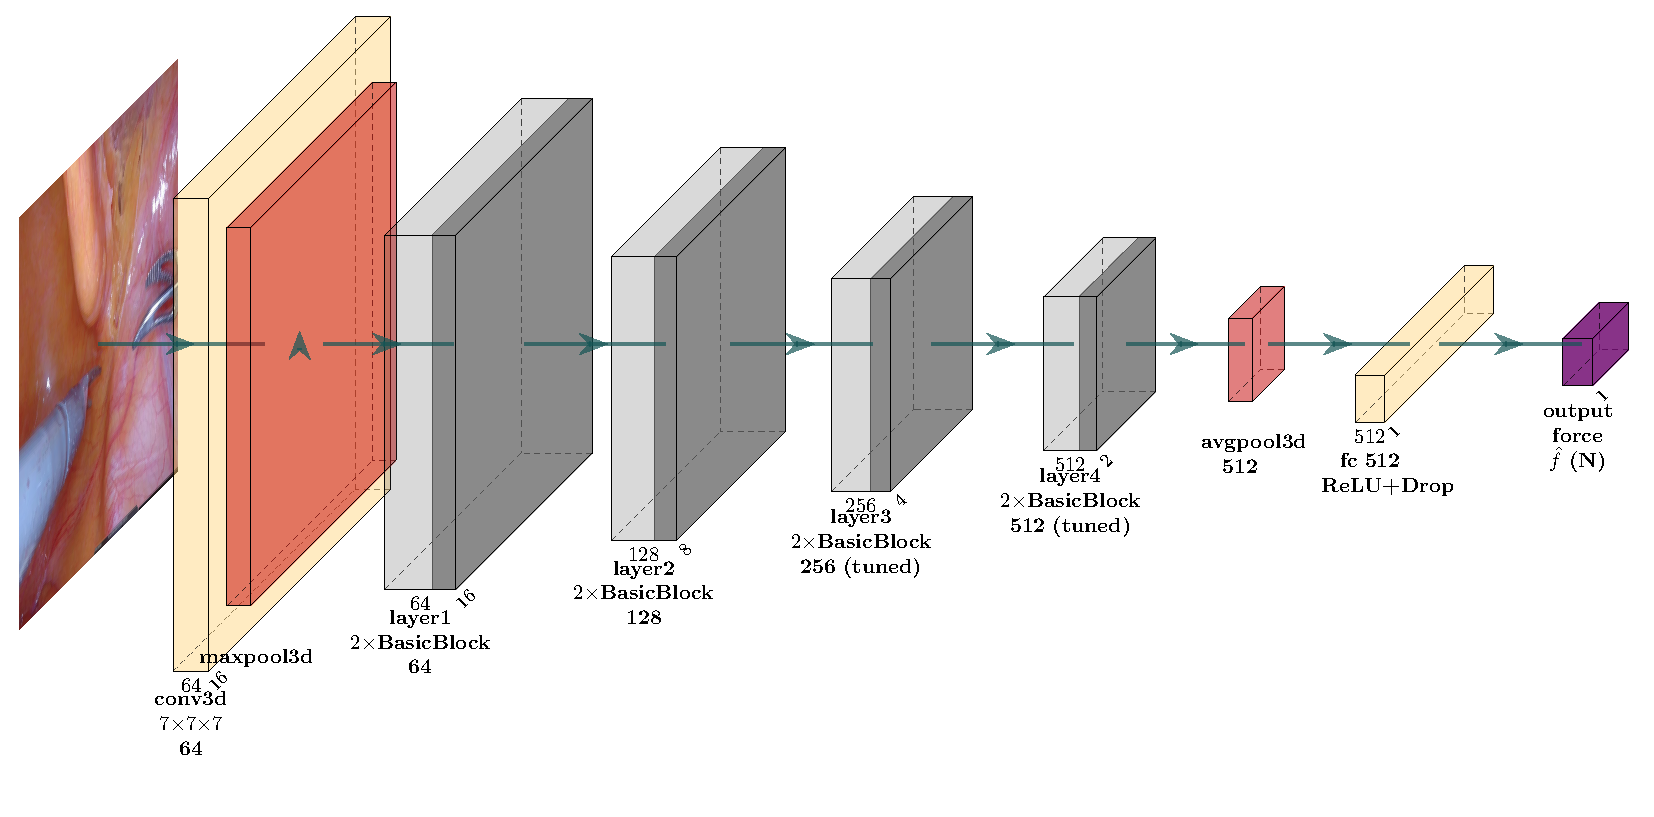
\includegraphics[width=\linewidth]{fig_forcenet.pdf}
\caption{Architecture of the unpublished video-based force estimator
(Eq.~\ref{eq:forcenet}). A 3D-ResNet (R3D-18) backbone processes the video
clip $3 \times T \times H \times W$ through a 3D-convolution stem and four
residual blocks (only the last two are fine-tuned), followed by global
average pooling and a two-layer regressor head
(Eq.~\ref{eq:forceloss}) that outputs the scalar force $\hat{f}$.}
\label{fig:forcenet}
\end{figure}

\subsection{Parameter provenance}
\label{sec:uq}
\begin{definition}[Parameter provenance]
\label{def:provenance}
A physical parameter $\theta$ carries a provenance tag
$\tau(\theta) \in \{\text{measured}, \text{estimated}, \text{assumed}\}$ and
a confidence $c(\theta) \in [0,1]$. A parameter is \emph{measured} when it
is acquired directly by a calibrated sensor, \emph{estimated} when it is
inferred by reconstruction or inverse simulation, and \emph{assumed} when
it is taken from a tissue-class table without case-specific evidence.
\end{definition}

Young's modulus uses a log-normal prior
$\log E \sim \mathcal{N}(\mu_0, \sigma_0^2)$, appropriate because tissue
stiffness spans orders of magnitude and must stay positive. A
Gaussian--Gaussian update combines the prior with deformation evidence in
closed form,
\begin{equation}
\sigma_{post}^{-2} = \sigma_0^{-2} + \sigma_{obs}^{-2}, \qquad
\mu_{post} = \sigma_{post}^{2}\left(\frac{\mu_0}{\sigma_0^{2}} + \frac{\mu_{obs}}{\sigma_{obs}^{2}}\right),
\label{eq:bayes}
\end{equation}
where $(\mu_{obs}, \sigma_{obs})$ summarize the deformation evidence. The
confidence is the fractional posterior narrowing,
$c = 1 - \sigma_{post}/\sigma_0$. For uncertainty propagation, a Laplace
approximation $p(\log E \mid \text{data}) \approx \mathcal{N}(\log E^*, H^{-1})$
with $H$ the Hessian of the negative log-posterior at the optimum is
sampled by Monte Carlo through the simulator to a 95\% prediction interval.

\subsection{Twin synchronization and simulation}
\label{sec:sync}
A digital twin is not a one-shot reconstruction but a continuously updated
copy \cite{landig2025}. Synchronization is the tracking loop: as each new
frame arrives, the tracker updates $\{\Delta_t\}$ on the fixed canonical
topology, and mechanical inversion can reuse the accumulated deformation as
additional inversion evidence.
Once constructed, the twin is used by driving $\mathcal{S}$ with new loads:
given a planned instrument trajectory $\{f_t^{plan}\}$, the simulator
produces the predicted deformation $\{u(E^*, \nu, f_t^{plan})\}$, which can
be rendered through the canonical field for visual rehearsal or post-processed
for quantities of interest (contact force, strain energy density, margin
strain). The audit modulates how these predictions are presented:
predictions are accompanied by intervals propagated from the corresponding
parameter uncertainties.

\begin{remark}[Optimization and learned components]
\label{rem:networkfree}
The Gaussian field is optimized as a set of per-primitive parameters, the
renderer is differentiable, and mechanical inversion optimizes physical
parameters through the simulator. The unpublished R3D-18 force estimator
is external to the twin and is used only to define the force-error model in
Sec.~\ref{sec:force}.
\end{remark}

\subsection{Use of generative AI tools}
During manuscript preparation, the authors used Cursor's AI-assisted
editor for English-language editing and LaTeX organization. Generative AI
was not used to generate data, conduct experiments, calculate metrics, or
draw scientific conclusions. The authors reviewed and approved all text
and remain responsible for the manuscript.

%% ===================================================================
\section{Conclusion}
\label{sec:conclusion}
%% ===================================================================
The proposed twin couples a canonical Gaussian surface representation with
fixed-correspondence tracking, force-aware mechanical parameterization, and
parameter provenance. Tracked Gaussians provide co-registered surface
motion and regional stiffness contrast for uninstrumented video; absolute
modulus is recovered only in known-force FEM experiments. The force-scale
identity explains why force uncertainty propagates to absolute modulus but
cancels in regional contrast. The experiments establish reconstruction and
tracking on public endoscopic data, a median background-modulus error of
4.3\% on six FEM scenarios, and a phantom contrast error of 6.9\% against
compression testing. The CT-derived liver mesh demonstrates geometry
construction from one de-identified clinical case. These results support
the proposed observation-to-simulation interface as a computational
method, but do not establish clinical performance or force-free
absolute-modulus recovery. Future work will require force-instrumented
tissue experiments, larger clinical datasets, and prospective evaluation
of task-specific simulation accuracy.



\section*{Abbreviations}
BRDF: bidirectional reflectance distribution function; CI: confidence
interval; CT: computed tomography; FEM: finite-element method; MPM:
material point method; NVS: novel-view synthesis; PSNR: peak
signal-to-noise ratio; RGB: red, green, and blue; SCARED: Stereo
Correspondence and Reconstruction of Endoscopic Data.

\section*{Declarations}

\subsection*{Ethics approval and consent to participate}
The public EndoNeRF, SCARED, finite-element benchmark, and \'ETS phantom datasets do not involve identifiable human subjects. The hospital computed tomography images are de-identified retrospective scans provided by Henan Provincial People's Hospital for geometry-source validation. No identifiable patient information is reported. Ethical review and approval were waived for this methodological study of de-identified imaging. Consent to participate was waived for the same reason.

\subsection*{Consent for publication}
Not applicable. The manuscript does not contain data from any identified individual person.

\subsection*{Availability of data and materials}
Project name: Soft-tissue digital twin.

Project home page: \url{https://github.com/liranyang123456-commits/soft-tissue-digital-twin}.

Operating system(s): Platform independent.

Programming language: Python.

License: MIT for the released pipeline code. The R3D-18 force estimator
used for the error model is unpublished and is not part of this
contribution.

The code, evaluation scripts, data-split definitions, aggregate force-error
parameters, and a README that generate the reported figures and tables are
available in that repository. EndoNeRF, SCARED, the finite-element
benchmark, and the \'ETS phantom are public datasets cited in this article.
The per-sample predictions from the ongoing, unpublished force-estimation
study are not part of this article; the aggregate parameters required for
the propagation experiment are included in the repository. The
de-identified hospital computed tomography images are not publicly
available because institutional consent restricts redistribution, but they
are available from the corresponding author on reasonable request.

\subsection*{Competing interests}
The authors declare that they have no competing interests.

\subsection*{Funding}
This work was supported by the National Natural Science Foundation of China (6240074117), the Henan University of Technology Young Backbone Teachers Training Program (21421329), the Open Project Program of the State Key Laboratory of Virtual Reality Technology and Systems (VRLAB2023C03), and the Cultivation Project of Tuoxin Team in Henan University of Technology (2024TXTD18). The funders had no role in study design, data collection, analysis, decision to publish, or preparation of the manuscript.

\subsection*{Authors' contributions}
RL conceived the study, developed the method, wrote the software, and drafted the manuscript. HM contributed the algorithm, software, and validation. ZL contributed validation, formal analysis, and multi-view evaluation. NW contributed clinical data curation and anatomical review. All authors read and approved the final manuscript.

\subsection*{Acknowledgements}
The authors thank Henan Provincial People's Hospital for providing the de-identified clinical computed tomography data used for the geometry-source validation.

\subsection*{Authors' information}
RL received the Ph.D. degree from Beihang University in June 2022 and is with Henan University of Technology. HM received the B.S. degree from Henan University of Technology and is with the same university. ZL is pursuing the Ph.D. degree at Beihang University. NW received the Ph.D. degree from Zhengzhou University in June 2021 and is with Henan Provincial People's Hospital.

\bibliography{references}

\end{document}
